% This is the Reed College LaTeX thesis template. Most of the work
% for the document class was done by Sam Noble (SN), as well as this
% template. Later comments etc. by Ben Salzberg (BTS). Additional
% restructuring and APA support by Jess Youngberg (JY).
% Your comments and suggestions are more than welcome; please email
% them to cus@reed.edu
%
% See https://www.reed.edu/cis/help/LaTeX/index.html for help. There are a
% great bunch of help pages there, with notes on
% getting started, bibtex, etc. Go there and read it if you're not
% already familiar with LaTeX.
%
% Any line that starts with a percent symbol is a comment.
% They won't show up in the document, and are useful for notes
% to yourself and explaining commands.
% Commenting also removes a line from the document;
% very handy for troubleshooting problems. -BTS

% As far as I know, this follows the requirements laid out in
% the 2002-2003 Senior Handbook. Ask a librarian to check the
% document before binding. -SN

%%
%% Preamble
%%
% \documentclass{<something>} must begin each LaTeX document
\documentclass[12pt,twoside]{reedthesis}
% Packages are extensions to the basic LaTeX functions. Whatever you
% want to typeset, there is probably a package out there for it.
% Chemistry (chemtex), screenplays, you name it.
% Check out CTAN to see: https://www.ctan.org/
%%
\usepackage{graphicx,latexsym}
\usepackage{amsmath}
\usepackage{amssymb,amsthm}
\usepackage{longtable,booktabs,setspace}
\usepackage{chemarr} %% Useful for one reaction arrow, useless if you're not a chem major
\usepackage[hyphens]{url}
% Added by CII
\usepackage{hyperref}
\usepackage{lmodern}
\usepackage{float}
\floatplacement{figure}{H}
% End of CII addition
\usepackage{rotating}

% Next line commented out by CII
%%% \usepackage{natbib}
% Comment out the natbib line above and uncomment the following two lines to use the new
% biblatex-chicago style, for Chicago A. Also make some changes at the end where the
% bibliography is included.
%\usepackage{biblatex-chicago}
%\bibliography{thesis}


% Added by CII (Thanks, Hadley!)
% Use ref for internal links
\renewcommand{\hyperref}[2][???]{\autoref{#1}}
\def\chapterautorefname{Chapter}
\def\sectionautorefname{Section}
\def\subsectionautorefname{Subsection}
% End of CII addition

% Added by CII
\usepackage{caption}
\captionsetup{width=5in}
% End of CII addition

% \usepackage{times} % other fonts are available like times, bookman, charter, palatino

% Syntax highlighting #22

% To pass between YAML and LaTeX the dollar signs are added by CII
\title{The spatial autocorrelation of fertility outcomes within England and Wales at the neighbourhood level}
\author{Ross Barker}
% The month and year that you submit your FINAL draft TO THE LIBRARY (May or December)
\date{2019/2020}
\division{Division of Social Statistics and Demography Social Sciences, Faculty of Social, Human and Mathematical Sciences}
\advisor{Dr.~Jason Hilton}
\institution{University of Southampton}
\degree{MSc Demography}
%If you have two advisors for some reason, you can use the following
% Uncommented out by CII
% End of CII addition

%%% Remember to use the correct department!
\department{Social Statistics and Demography Social Sciences}
% if you're writing a thesis in an interdisciplinary major,
% uncomment the line below and change the text as appropriate.
% check the Senior Handbook if unsure.
%\thedivisionof{The Established Interdisciplinary Committee for}
% if you want the approval page to say "Approved for the Committee",
% uncomment the next line
%\approvedforthe{Committee}

% Added by CII
%%% Copied from knitr
%% maxwidth is the original width if it's less than linewidth
%% otherwise use linewidth (to make sure the graphics do not exceed the margin)
\makeatletter
\def\maxwidth{ %
  \ifdim\Gin@nat@width>\linewidth
    \linewidth
  \else
    \Gin@nat@width
  \fi
}
\makeatother

%Added by @MyKo101, code provided by @GerbrichFerdinands

\renewcommand{\contentsname}{Table of Contents}
% End of CII addition

\setlength{\parskip}{0pt}

% Added by CII

\providecommand{\tightlist}{%
  \setlength{\itemsep}{0pt}\setlength{\parskip}{0pt}}

\Acknowledgements{
Thank you to my dissertation supervisor Dr.~Jason Hilton for guiding and supporting this research. Thanks is also due to those who have published R code online relating to spatial econometrics.
}

\Dedication{

}

\Preface{

}

\Abstract{
The influence of space on fertility is unclear, while the influence of compositional and contextual determinants are more clearly understood. At the local level within England and Wales, fertility varies vastly from lowest-low fertility to levels well above replacement level. Using small-scale, neighbourhood-level data on socio-demographic, economic and contextual conditions, this dissertation aims to isolate and explain the role of spatial influence and contagion on fertility. Methodologically, Ordinary Least-Squares regression is compared to four spatial models: the Spatial Lag Model, Spatial Error Model, Spatial Durbin Model and Spatial Durbin Error Model. Theoretically, the diffusion of ideals and norms is cemented in demographic approaches to fertility change. This approach is followed here, namely through the role of social networks and the small-scale transmission of ideas and norms. Education, ethnicity, income, population density, divorce prevalence, social support and non-religiousness test significant, with university-level education and ethnicity hosting the greatest improvements in model performance. The inclusion of endogenous and exogenous spatial components vastly improves explanatory power, that is, including dependence between neighbourhoods both in relation to fertility behaviours and the explanatory variables. However, she sub-regional analysis of spatial processes requires further research in isolating the exact role of social contagion on fertility.

\par

\textbf{Keywords}: fertility, spatial dependence, spatial autocorrelation
}

	\usepackage{pdflscape}
\newcommand{\blandscape}{\begin{landscape}}
\newcommand{\elandscape}{\end{landscape}}
	\usepackage{booktabs}
\usepackage{longtable}
\usepackage{array}
\usepackage{multirow}
\usepackage{wrapfig}
\usepackage{float}
\usepackage{colortbl}
\usepackage{pdflscape}
\usepackage{tabu}
\usepackage{threeparttable}
\usepackage{threeparttablex}
\usepackage[normalem]{ulem}
\usepackage{makecell}
% End of CII addition
%%
%% End Preamble
%%
%
\begin{document}

% Everything below added by CII
  \maketitle

\frontmatter % this stuff will be roman-numbered
\pagestyle{empty} % this removes page numbers from the frontmatter
  \begin{acknowledgements}
    Thank you to my dissertation supervisor Dr.~Jason Hilton for guiding and supporting this research. Thanks is also due to those who have published R code online relating to spatial econometrics.
  \end{acknowledgements}

  \hypersetup{linkcolor=black}
  \setcounter{tocdepth}{2}
  \tableofcontents

  \listoftables

  \listoffigures
  \begin{abstract}
    The influence of space on fertility is unclear, while the influence of compositional and contextual determinants are more clearly understood. At the local level within England and Wales, fertility varies vastly from lowest-low fertility to levels well above replacement level. Using small-scale, neighbourhood-level data on socio-demographic, economic and contextual conditions, this dissertation aims to isolate and explain the role of spatial influence and contagion on fertility. Methodologically, Ordinary Least-Squares regression is compared to four spatial models: the Spatial Lag Model, Spatial Error Model, Spatial Durbin Model and Spatial Durbin Error Model. Theoretically, the diffusion of ideals and norms is cemented in demographic approaches to fertility change. This approach is followed here, namely through the role of social networks and the small-scale transmission of ideas and norms. Education, ethnicity, income, population density, divorce prevalence, social support and non-religiousness test significant, with university-level education and ethnicity hosting the greatest improvements in model performance. The inclusion of endogenous and exogenous spatial components vastly improves explanatory power, that is, including dependence between neighbourhoods both in relation to fertility behaviours and the explanatory variables. However, she sub-regional analysis of spatial processes requires further research in isolating the exact role of social contagion on fertility.
    
    \par
    
    \textbf{Keywords}: fertility, spatial dependence, spatial autocorrelation
  \end{abstract}

\mainmatter % here the regular arabic numbering starts
\pagestyle{fancyplain} % turns page numbering back on

\hypertarget{introduction}{%
\chapter*{Introduction}\label{introduction}}
\addcontentsline{toc}{chapter}{Introduction}

The influence of space has been studied at the micro, meso and macro level in addressing all areas of fertility. The aggregate scale partly loses individual-level processes, but the individual scale lacks geographical detail to measure diffusion over space. Demography has long being referred to as a spatial social science (Voss, \protect\hyperlink{ref-voss2007}{2007}), and the role of space appears to be increasingly complicated and heterogenic, and becoming increasingly studied within Demography. The ideas of a neighbour and neighbourhood are used in this dissertation as the agents in the spatial processes of fertility. A neighbourhood is a collection of individuals and households who host similarities in proximity and sociodemographic traits. Due to neighbourhood proximity, individuals within bordering neighbourhoods influence one another through communication. Currently, the scale of high-quality data available for fertility research is mostly at the individual, social network, regional and national level, with a previously lacking middle-ground of `neighbourhood'. Here the neighbourhood is taken to be a Middle Super Output Area (MSOA), of which there are 7,201 in England and Wales, and defined as areas of roughly 7,800 individuals and a median size of 3.3km2 in 2011. Both England and Wales have avoided the falls in Total Fertility Rate (TFR) that lead to panic regarding population ageing and decline as seen in Central Europe, Southern Europe and East Asia. When discussing national outcomes, micro and meso processes are confounded into a TFR that paints a clear but often misleading picture; and examining within-country and within-region variation clarifies the determinants of fertility intentions and behaviours.

In approaching the analysis of fertility from the neighbourhood scale, the spatial processes, and apparent effects of non-spatial determinants of fertility differ than when measured regionally or nationally. Caveats to fertility-based research are dependent on the type of data used. The neighbourhood scale reduces the gap between the individual and the aggregate, allowing for space to be included within a model that is more detailed than the regional, but less detailed than the household level. The change of level is closer to the processes of spatial interaction and diffusion that a regional approach overlooks and potentially misidentifies. By doing so, the aggregation of households and individuals to the neighbourhood level leads to diffusion of ideas being measurable. Dependent on diffusion processes, communication itself is tentatively expected to aid in the understanding of regional patterns. This communication and social network effects are summarised by the term `social contagion'.

Regional patterns aid in the explanation of national outcomes (Snyder, \protect\hyperlink{ref-snyder2001}{2001}). Focus on the regional has long-been practiced and is deemed important within Demography (Watkins, \protect\hyperlink{ref-watkins2014}{2014}), yet, the sub-regional scale of analysis is not equally studied, perhaps due to lack of data or the assumption of grandiose processes that need to be explored on the small-scale. While many regional European studies have modelled the spatial dependency of fertility, geographies and methodologies are not sufficient in addressing the social networks central to diffusionist theory. Often, important model diagnostics appear to be excluded from the spatial model-building processes. Diffusion is largely associated with fertility decline, yet, ongoing social network effects are both negative and positive. Sub-regional analysis, and the comparison of model performance, is expected to aid in the regional, and in turn, national explanations of fertility.

In testing the accuracy of statements above, individual-level census data is used to source six of the seven explanatory variables used in this dissertation. The other variable, Income, is an estimation sourced from the Office for National Statistics (ONS). The number of births by area and age are also sourced from the ONS through birth registration data. The modelling is restricted to the year 2011 due to the reliance on census data. The model-building process is not only led by reasoning relating the spatial element of fertility; the lack of a spatial term within Ordinary Least-Squares (OLS) regression violates the assumption that each observation is independent of other observations. Spatial models are necessary when using sub-regional aggregate data with neighbours particularly when fertility is heavily influenced by space. The appropriate models tested here are four autoregressive models, with the spatial element being related to the dependent variable (endogenous interaction effects), the error in the model (interaction effects in the error term), the explanatory variables (exogenous interaction effects) or a combination/hybrid of multiple. The variables included in the model are: university-educated women, high-TFR ethnicities, net weekly income, population density, prevalence of divorce, social housing and non-religiousness.

There are few examples of research at this scale particularly within the United Kingdom (UK), while European Union (EU) wide approaches are common. Previous research using spatial modelling largely addresses historical demography and the diffusion of norms. Regional-level models including spatial interactions in current research are often limited, but do show the significant diffusion of fertility trends between regions with various spatial models (Campisi, Kulu, Mikolai, Klüsener, \& Myrskylä, \protect\hyperlink{ref-campisi2020}{2020}; Vitali \& Billari, \protect\hyperlink{ref-vitali2017}{2017}; Waldorf \& Franklin, \protect\hyperlink{ref-waldorf2002}{2002}). Despite many model options, the Spatial Lag model, also called the mixed regressive-spatial autoregressive model takes a forefront in analyses.

The primary aim of this dissertation is to identify to what extent low-level geography matters in understanding fertility through spatial autocorrelation, a term interchangeable with spatial dependence. That is, I am to identify how one neighbourhood `affects' its neighbour. I tentatively hypothesise that spatial dependence will not be eliminated by the addition of variables above into an OLS model, and that including the spatial autocorrelation of TFR within the model will be necessary and methodologically sound. This dissertation is structured as follows. Following a summary of the literature (2), the aims and objectives (3) look back to the previous section and identify unanswered questions. The variables to include within the model are then collected and justified (4). The data sources and calculations (5 \& 6) follow with the formulae and tests necessary in spatial econometrics. The results (7) are structured by the descriptive results, three research questions and a comparison of the models' capabilities. Finally, the limitations (8) and discussion (9) bring together the results alongside the individual research questions in line with the model of best-fit.

\hypertarget{Review}{%
\chapter{Literautre Review}\label{Review}}

Individual characteristics such as education and income are associated with fertility intentions and outcomes. The processes leading to differences in fertility outcomes by individual characteristics influence the size of the gap between fertility intentions and outcomes. Social network processes are underlying determinants of the fertility gap, influencing different individuals to varying degrees in addition to underlying individual characteristics. The analysis of such network processes is undertaken both on the small- and large-scale. Small-scale analyses require thorough qualitative sources and complex modelling. Growing analysis of regional fertility is taking place in Europe, particularly with a focus on education (Wood, Klüsener, Neels, \& Myrskylä, \protect\hyperlink{ref-wood2020}{2020}) and income (Campisi et al., \protect\hyperlink{ref-campisi2020}{2020}; Nisén et al., \protect\hyperlink{ref-nisen2020}{2020}). Despite the growth in the two scales, the sub-regional, local scale remains relatively unexplored. The current literature is addressed by three sections. First, the processes of social networks at the interpersonal level; second by diffusion at the large scale; and finally the connection of the two scales to form an overarching theory.

\hypertarget{small-scale-diffusion}{%
\section{Small-Scale Diffusion}\label{small-scale-diffusion}}

The transmission of fertility norms, ideals and intentions occurs on a hierarchical scale; the first level is the individual, and the final is the nation. Leaving the aggregate scale and focussing on the individual, the family, friends, and workplace acquaintances form a personal network unique to each individual. In a landmark paper, Watkins (\protect\hyperlink{ref-watkins1995}{1995}) addresses social interaction and networks as influencing reproductive behaviour. Watkins argues that not only the spread of new technologies and the diffusion of ideas are important in fertility decline, but also the personal networks of individuals. In further clarity,Bongaarts \& Watkins (\protect\hyperlink{ref-bongaarts1996}{1996}) argue that diffusion is an independent actor that leads to changes in fertility behaviour, as social interaction produces new ideas relating to childbearing as a variable of its own. The authors emphasise how information is exchanged and thereafter enforced or encouraged. That is, changes in fertility occur due to structural change, and diverge from the Second Demographic Transition (SDT), which largely focusses on the individual, while lacking acknowledgement of social networks (Bernhardt, \protect\hyperlink{ref-bernhardt2004}{2004}). Bernardi \& Klärner (\protect\hyperlink{ref-bernardi2014}{2014}) also note the delayed adoption of social network theory in the Global North due to the assumption that in individualistic societies, social considerations are not effective in influencing childbearing intentions. That is, small- and large-scale analyses of diffusion remain somewhat separate and scale-dependent despite relying on the same underlying processes.

Building upon the above theoretical developments and with high-quality data, Balbo \& Barban (\protect\hyperlink{ref-balbo2014}{2014}) find fertility behaviour to be influenced by friendship circles. If an individual has a friend who has children, the risk of having a child himself/herself increases, yet 2 years following the birth of a friend's child, network effects begin to diminish. The friendship influences on fertility appear to increase with age to 28 years old, with declining influence of social networks thereafter, thereby noting the temporal and variant nature of social network effects. The contagion between friends and members of a network is also developed by Lois \& Arránz Becker (\protect\hyperlink{ref-lois2014}{2014}) who emphasise the process of `social contagion' combining three different social network effects: social learning, social pressure, and social opportunity cost. In comparison, Bernardi \& Klärner (\protect\hyperlink{ref-bernardi2014}{2014}) identify social learning, social pressure, social contagion and social support as drivers of fertility change, with overarching points of interdependence. The exact processes and wording differ, but the overarching process remain unchanged. Social contagion is present within networks of people, and leads to differences in intended and actual fertility.

As social interactions occur at the interpersonal scale, the measurement and significance of such relationships is most appropriate at the micro level. In a comparative study of West and East Germany, Bernardi, Keim, \& Von Der Lippe (\protect\hyperlink{ref-bernardi2007}{2007}) identify two elements of fertility decision-making, firstly `individual and structural characteristics of networks' and `social mechanisms' between individuals at the core. In the same study of 54 people, network size varies between 14 and 17. The actual agents enabling exchange of ideas relating to childbearing are the social mechanisms within the social network. Bernardi et al. (\protect\hyperlink{ref-bernardi2007}{2007}) also note the complexities such as heterogeneity in network structures, and differences between geography and gender. Measuring these is difficult, with few surveys being able to answer hypotheses of social interaction due to lack of depth and network (Rossier \& Bernardi, \protect\hyperlink{ref-rossier2009}{2009}).

The endogenous networks that carry information and further the transition to parenthood have been tested with agent-based simulation models. For example, social interactions affecting first-birth probabilities for Austrian women (Diaz, Fent, Prskawetz, \& Bernardi, \protect\hyperlink{ref-diaz2011}{2011}). In a comparative agent-based modelling approach, Nomes and colleagues (2019) use Belgian census data to show that the two-child family norm and the homogenisation of this ideal throughout the country led to rising as well as falling fertility in different parts of Belgium. Fent, Diaz, \& Prskawetz (\protect\hyperlink{ref-fent2013}{2013}) also use agent-based modelling by incorporating agents' heterogeneity and network structure, and find a positive association between network size and fertility outcomes.

Only small-scale, qualitative studies can capture the origins of social contagion, while the grander process of diffusion across space can grasp at the outcomes of such processes. The literature has shown that individual characteristics are not sufficient in identifying the processes that lead to fertility intentions and outcomes, but rather, the social processes between individuals, groups and neighbourhoods are significant and should not be overlooked. Without being able to model individuals, the inclusion of a spatial term at the aggregate level closely mimics the missing link of neighbour-to-neighbour contagion. In sum, the influence of social networks can and should be tested at the aggregate scale, but the complexity and requirement of assumptions is not understated.

\hypertarget{large-scale-diffusion}{%
\section{Large-Scale Diffusion}\label{large-scale-diffusion}}

Despite the theoretical reliance on interpersonal contagion, the sources of data within this research require aggregation. Since the pivotal works regarding the fall in fertility in the Global North during the latter half of the 20th century (Lesthaeghe, \protect\hyperlink{ref-lesthaeghe1995}{1995}; Van De Kaa, \protect\hyperlink{ref-vandekaa1987}{1987}), aggregate-level diffusion has been tested within Demography. Despite criticisms of the SDT relating to simplification and a false permanence (Szreter, \protect\hyperlink{ref-szreter1993}{1993}), the underlying processes that underpin the theory remain relevant and mainstream (Casterline \& Washington, \protect\hyperlink{ref-casterline2001}{2001}). The ability of women to pursue careers above raising children is central to the SDT, based in individualism and women's agency in relation to childbearing (Becker, \protect\hyperlink{ref-becker1981}{1981}; Van De Kaa, \protect\hyperlink{ref-vandekaa1987}{1987}). The ideals of the SDT have already spread throughout England, and the individualism that is now common challenges social network effects routed in community. Therefore, there is a slight disconnect between the previous and current sections, and the hangovers of the SDT fertility-decline based theory are not as relevant as previous, yet, the diffusion processes are.

Casterline \& Washington (\protect\hyperlink{ref-casterline2001}{2001}) cites three bodies of work forwarding the grand theory of diffusion: the first being behavioural innovation (such as fertility control), the second is derived from the ``innovation diffusion'' concept led by ideational theories. The third is based in social dynamics, relating to the channels by which the two former dynamics forward the spread of behaviours and ideas. While focussing on social dynamics, Casterline \& Washington (\protect\hyperlink{ref-casterline2001}{2001}) terms social effects as effects derived largely from social learning and social influence. Social, interpersonal effects are therefore at the core. This model of social effects bares the simple premise ``changes in the knowledge and behaviours of some individuals affect the likelihood that other individuals will change their knowledge and/or behaviours'' (Casterline \& Washington, \protect\hyperlink{ref-casterline2001}{2001}, p. 17). Manski (\protect\hyperlink{ref-manski1993}{1993}) clarifies with three effects; with endogenous relating to social interactions; contextual being the group in which one resides; and correlated being similarities between individuals in similar environments (Durlauf \& Walker, \protect\hyperlink{ref-durlauf2001}{2001}).

Klüsener, Neels, \& Kreyenfeld (\protect\hyperlink{ref-klusener2013}{2013}) are one of the first examples to use sub-national scale in spatially modelling TFR, where the diffusion of non-marital fertility behaviours are influenced by external and internal borders from 1960 to 2007. The diffusion of socioeconomic norms and values, based on the Easterlin supply and demand hypothesis is shown in Italy from 1952 to 1995 through a Spatial Lag model (Waldorf \& Franklin, \protect\hyperlink{ref-waldorf2002}{2002}). This approach, by Waldorf \& Franklin (\protect\hyperlink{ref-waldorf2002}{2002}) spatially models 18 regions, ending with an adjusted R2 value of 0.9, which raises more concern than confidence as diffusion of fertility behaviour is unlikely to explain the vast majority of child-bearing decisions. In a comparable paper to this dissertation, Campisi et al. (\protect\hyperlink{ref-campisi2020}{2020}) compare three spatial autocorrelation regression models, two multilevel models, and OLS, concluding that the Spatial Lag model is the most appropriate to the data and phenomena at play. The variables included in the model are TFR, population density (log scale), share of apartment housing, Gross Domestic Product (GDP) per capita, employment rate, share of employment in agriculture and prevalence of divorce. Spatial autocorrelation of residuals decreases from the OLS model to the Spatial Lag Model, the Spatial Error Model and the Spatial Durbin Model. Despite being highly relevant, the approach lacks diverse non-economic variables that may account for spatial autocorrelation such as ethnicity. In addition, the authors do not show diagnostics tests such as the Robust Larange Multiplier test, which may disprove the existence of endogenous interaction effects. Analysing the residuals of autoregressive models is not useful, as a vast fall in residual spatial autocorrelation is certain when including spatial autoregression in the model formula. Vitali \& Billari (\protect\hyperlink{ref-vitali2017}{2017}) also approach the data similarly, by testing fertility diffusion through the time frame 1991 to 2010 in 110 regions of EU. In addition to using two spatial models, Vitali and Billari find the spatial element of fertility to remain when controlling for significant socio-demographic variables, but with only four variables included.

At the opposite scale, very-low level analysis of fertility is rare. Within fertility research, a model including a spatial term below the regional level has not, to my knowledge, been done. For instance, Basten, Huinink, \& Klüsener (\protect\hyperlink{ref-basten2011}{2011}) model the convergence of fertility trends in Austria, Germany and Switzerland alongside a very-low level analysis of Bremen, Germany. Yet, no spatial element is included within the model. While this dissertation focusses on England and Wales, a similar working paper by Boyle, Graham, \& Feng (\protect\hyperlink{ref-boyle2007}{2007}) fills a geographical gap by modelling fertility clusters in Scotland, split into 10,000 neighbourhoods. A smaller scale is used when compared to this dissertation; Consistent Areas Throughout Time (CATTs), which enables a comparison of census data from between 1981, 1991 and 2001. Despite a fine geography, the models lack a spatial element, and the use of CATTs result in areas with very few people and births. As is common in small-scale analyses, crude geographic aggregations are often used within these papers (Boyle et al., \protect\hyperlink{ref-boyle2007}{2007}). The lack of data with well-justified boundaries, as in the case of CATTs, separated by population alone, leads to the identification of spatial autocorrelation that may be due to one area being split in two.

Within the UK, few papers have modelled fertility with a spatial principle. In multiple works based in the UK, the size of the settlement, population density and selective migration, which is based on fertility intentions, are significant to fertility (Kulu, \protect\hyperlink{ref-kulu2013}{2013}; Kulu \& Boyle, \protect\hyperlink{ref-kulu2009}{2009}; Kulu \& Vikat, \protect\hyperlink{ref-kulu2007}{2007}; Kulu \& Washbrook, \protect\hyperlink{ref-kulu2014}{2014}). The methodologies of Kulu and UK-based spatial analysis largely remain within hazard models and avoiding the retention of neighbourhood boundaries through aggregation. Fiori, Graham, \& Feng (\protect\hyperlink{ref-fiori2014}{2014}) use a hazard model to predict outcomes for five agglomerated geographies by rural and urban context, concluding that geography is relevant to first births, but not higher order births. The base geography is Lower Super Output Area (LSOA), and the issue of using such a small geography is overcome by the merging the data. Jaadla, Reid, \& Garrett (\protect\hyperlink{ref-jaadla2018}{2018}), in a larger-scale geography to Fiori and colleagues, identify the fertility transition in England and Wales between 1851 and 1911 beginning in areas of high population and high technological density, such as cotton mill towns in the North West. In the early 20th century and 2001/2011 context of London, Jaadla et al.~(2020) are working on a spatial model including general fertility rate as the dependent variable, and population density, share of married women, share of managers, share of elementary occupations and share of foreign born as explanatory variables. Jaadla and colleagues use the 624 wards of London in the latter data frame. Similar to Jaadla et al. (\protect\hyperlink{ref-jaadla2018}{2018}), historic modelling has identified the fertility transition processes in Sweden and Prussia, but with greater attention to spatial processes both in theory and in model formulae. Klüsener, Dribe, \& Scalone (\protect\hyperlink{ref-klusener2019}{2019}) model fertility in Sweden from 1880 to 1900, finding the diffusion of fertility decline was less spatially clustered in elite communities than in the poor communities, that is, the elite led the fertility decline and through quicker corridors of communication. In a similar vein, Goldstein \& Klüsener (\protect\hyperlink{ref-goldstein2014}{2014}) identify corridors of fertility diffusion in Prussia, utilising spatial autocorrelation determinants in identifying spatial clustering, and testing the presence of autocorrelation through the omission of variables. Both papers argue for greater attention to geographic location, and spatial approaches have grown in prominence but largely remained at the regional level.

\hypertarget{conclusion-literature-review}{%
\section{Conclusion: Literature Review}\label{conclusion-literature-review}}

Some research has shown that the inclusion of and complication caused by spatial dependence is often unnecessary, and modelling aggregate fertility without a spatial element yields useful results (Bujard \& Scheller, \protect\hyperlink{ref-bujard2017}{2017}; Fox, Klüsener, \& Myrskylä, \protect\hyperlink{ref-fox2019}{2019}; Hank, \protect\hyperlink{ref-hank2001}{2001}; Sobotka \& Adigüzel, \protect\hyperlink{ref-sobotka2002}{2002}). Such approaches can also avoid violating the OLS assumption of non-dependence, as influence between regions can often be considered similarly to the influence between countries at such large scales. The scale of such studies is also an understated disadvantage, in capturing what are in essence social network effects at the relatively large geographic NUTS-3 sub-national division. Within this sub-national setting, populations range from 150,000 to 800,000. Country diagnostics are potentially too grand to display individual behaviour (Bryan \& Jenkins, \protect\hyperlink{ref-bryan2016}{2016}), and this literature review has also found regional diagnostics to be too grand to display individual behaviour. Both the regional and national approaches incur a far departure from the micro and meso scale where fertility-related decision-making takes place. That is, social contagion occurs in the individual and interpersonal space where ideas are formed, norms expected and behaviours encouraged or discouraged, and remaining closely tied to this meso level allows the outcomes of spatial processes to be measured.

The overarching processes of fertility change are spatial and interpersonal; processes captured at the neighbourhood scale more so than the regional or national. There are two relevant gaps in the literature addressing the processes of spatial diffusion. First, UK-specific research is limited. Although Local Authorities have been used in analysing TFR, these papers are largely descriptive, with the use of spatial autocorrelation rarely used (with the exception of Walford and Kurek, 2016). Second, an exploration of model types at the sub-regional, local scale is very rare. Spatial sub-national analyses often include economic factors within the models (e.g.~Nisén et al., \protect\hyperlink{ref-nisen2020}{2020}), but lack important variables such as ethnicity. The intention of the following sections is therefore to build an analytical analysis of local fertility taking into account previous research.

\hypertarget{Aims}{%
\subsection{Aims and objectives}\label{Aims}}

The overarching aim of this dissertation is to identify whether fertility diffusion is present at the MSOA level within England and Wales. That is, the exchange of fertility behaviour between neighbourhoods. Three questions, which also form the oncoming results section of this dissertation are therefore as follows, followed by the research aims addressing the research questions:\\
\hspace*{0.333em}

\textbf{Descriptive}: Is there spatial autocorrelation in fertility outcomes, and if so, has this weakened or strengthened over time (from 2002-2018)?

~

\textbf{Theoretical}: If existent, does spatial autocorrelation remain when accounting for compositional and contextual determinants?

~

\textbf{Methodological}:
Does the inclusion of a spatial autoregressive element to base OLS formula aid in the explanatory power of small-scale fertility outcomes, signifying the necessary inclusion of neighbour-to-neighbour fertility diffusion?

~
\begin{enumerate}
\def\labelenumi{\arabic{enumi}.}
\tightlist
\item
  Test for spatial autocorrelation in Age-Specific Fertility Rates (ASFRs) and TFR from 2002 to 2018.
  \begin{enumerate}
  \def\labelenumii{\roman{enumii})}
  \tightlist
  \item
    Calculate Global Moran's I and illustrate Local Moran's I.
    ~
  \end{enumerate}
\end{enumerate}
\begin{enumerate}
\def\labelenumi{\arabic{enumi}.}
\setcounter{enumi}{1}
\tightlist
\item
  Build an OLS model and examine the spatial autocorrelation of model residuals in the addition of each variable.
  \begin{enumerate}
  \def\labelenumii{\roman{enumii})}
  \tightlist
  \item
    Add the seven variables stepwise.
  \item
    Use spatial tests to identify which model is best-fitted.

    ~
  \end{enumerate}
\item
  Build four spatial autocorrelation models to test the neighbour-to-neighbour diffusion hypothesis.
  \begin{enumerate}
  \def\labelenumii{\roman{enumii})}
  \tightlist
  \item
    Spatial Lag Model (SAR), Spatial Error Model (SEM), Spatial Durbin Model (SDM) and Spatial Durbin Error Model (SDEM).
  \item
    Describe the most appropriate final model results and implications.
  \end{enumerate}
\end{enumerate}
\hypertarget{Analytical}{%
\chapter{Analytical Strategy}\label{Analytical}}

Socio-demographic characterises are paramount in the pre-emptive and time-specific intention to have a child, as well as the ability to meet these intentions (Schoen, Astone, Kim, Nathanson, \& Fields, \protect\hyperlink{ref-schoen1999b}{1999}). Constraints to achieving fertility goals are largely measurable through the use of socio-demographic individual and couple-level characteristics. Grand fertility differentials within England and Wales do not occur in a generalisable North versus South or East versus West duality as in Italy or Germany. This grand view hides the largest differentials that lie within the region at the very-small scale, defined here as below the Local Authority level. As the previous section analysed the main authors and ideas, this section analyses the existence of variable-specific fertility relationships. In doing so, this section is structured first by an exploration of individual-level fertility determinants. The second section will analyse neighbourhood measures of fertility, building upon the individual-level data. The third and final section will discuss spatial influence and how this can be measured.

\hypertarget{composition-effects}{%
\section{Composition effects}\label{composition-effects}}

\textbf{Age}: Age determines childbearing biologically and also in relation to the influence of socio-demographics, with the mean age of childbearing increasing within England and Wales from a low of 26.4 in 1973 to 30.5 in 2017 (ONS, 2019). The postponement of childbearing led to a temporary decrease in TFR in the late 1990s and early 2000s, yet this effect in TFR ended around 2010 with tempo-adjusted TFR showing a gradual and non-extreme decline in European fertility, largely recovering from the postponement effects by 2007 (Goldstein, Karaman Örsal, Kreyenfeld, \& Jasilioniene, \protect\hyperlink{ref-goldstein2013}{2013}). Therefore, the influence of postponement and transitioning age of first birth are not expected to have a large impact on fertility, although this may differ by locality. The presence of postponement varies by socio-economic background, however, with education being directly linked to postponement (Blossfeld \& Huinink, \protect\hyperlink{ref-blossfeld1991}{1991}; Ní Bhrolcháin \& Beaujouan, \protect\hyperlink{ref-nibhrolchain2012}{2012}). Postponement is not included in the model explicitly, but is likely to be captured by the measurement of TFR itself as well as proxy determinants of postponement, namely education.

\textbf{Education}: Education is sometimes considered a central demographic determinant after age and sex (Lutz \& Samir, \protect\hyperlink{ref-lutz2011}{2011}). Recently, the cohort fertility behaviours of Generation Xers (born mid-1960s to early 1980s) have shown a marked increase in the fertility of women of university-level education in the United States (Zang, \protect\hyperlink{ref-zang2019}{2019}). The Nordic countries also display a lessening of the negative education-fertility outcomes, with those more socially disadvantaged being childless in higher proportions (Jalovaara et al., \protect\hyperlink{ref-jalovaara2019}{2019}). The negative association between education and fertility may be lessening in certain sub-groups and contexts, however, the fertility outcomes of British university-educated women is below replacement level and below that of non-university educated women (Testa, \protect\hyperlink{ref-testa2014}{2014}; Wood, Neels, \& Kil, \protect\hyperlink{ref-wood2014}{2014}); by age 46 there is a strong negative association between education and reaching stated fertility intentions (Berrington \& Pattaro, \protect\hyperlink{ref-berrington2014}{2014}). Education may also be viewed as interacting with contextual norms, in that highly-educated groups benefit disproportionately from work-family reconciliation programmes as well as in geographic areas where combining work and life is the norm (Wood et al., \protect\hyperlink{ref-wood2020}{2020}). The pattern in the UK still clearly displays lower fertility for those who have higher education, while education may also host broad contextual effects, therefore, a negative association is expected, countered by potential contextual effects leading to increased fertility.

\textbf{Income}: The role of wealth on fertility, most frequently measured with GDP per capita, has changed in previous decades; as GDP per capita is now positively associated with TFR in high-income settings such as the EU (Fox et al., \protect\hyperlink{ref-fox2019}{2019}; Myrskylä, Kohler, \& Billari, \protect\hyperlink{ref-myrskyla2011a}{2011}). Macro-level research is on the regional and national scale, with high- and low-fertility contexts pinpointed such as wealthy Northern Europe and austerity-hit Southern Europe, however, the within-country differences are expected to be stark and not as closely linked to the positive association seen on a continental scale. Income may reduce the perceived costs of childbearing, allowing work and family life to be combined. However, in a high-income household, the loss of work to care for a child results in a relatively large monetary loss. The cost-benefit analysis may therefore be influenced by local geography as employment conflicts more so with childbearing in contexts that are less gender-egalitarian. Collinearity may also influence results, that is, the concentration of highly-educated individuals creates concentrated economically advanced areas (Fox et al., \protect\hyperlink{ref-fox2019}{2019}). The sub-regional relationship between income and fertility is expected to be negative, even though the UK is within a high-fertility and high-income setting when viewed from in the European, national context.

\textbf{Ethnicity}: The fertility of immigrants is generally higher than non-immigrant fertility, although the two become similar over time (Dubuc, \protect\hyperlink{ref-dubuc2012}{2012}). A more appropriate approach than measuring international migration is by measuring proportion of certain high fertility ethnic groups within the population. From 2000 to 2006 using the Labour Force Survey, Dubuc (\protect\hyperlink{ref-dubuc2009}{2009}) estimated the white British female population to have a TFR of 1.73, similar to White Other, Black Caribbean and Indian populations, with Chinese women having very-low TFR (1.20). Black African, Pakistani and Bangladeshi female populations hosted TFRs above replacement level (2.40, 2.85, and 3.12 respectively). Dubuc also note religious differences within the Indian ethnicity, with Muslims hosting higher TFR than Hindus, and Sikhs less so than Hindus. These findings relate to TFR, but cohort fertility rates also show significant differences between the immigrants and native-born populations (Wilson, \protect\hyperlink{ref-wilson2020}{2020}). An interesting outcome may result from the migrants normally migrating to wealthy areas, and low-fertility contexts (Billari \& Dalla-Zuanna, \protect\hyperlink{ref-billari2012}{2012}). The neighbourhood scale may capture the low-level differences, such as an immigrant enclave within a wealthy Local Authority. In line with Dubuc's findings, high proportions of women in the Black African, Pakistani and Bangladeshi ethnic groups are expected to lead to higher TFR.

\hypertarget{contextual-effects}{%
\section{Contextual effects}\label{contextual-effects}}

\textbf{Population density}: The urban-rural simplified dichotomy is proven to be significant in most countries, and here, population density is used as a proxy for the urbanisation of a neighbourhood. The UK is not isolated in hosting higher fertility in less populated areas as shown by Fiori et al. (\protect\hyperlink{ref-fiori2014}{2014}), but also in high-income countries such as the Netherlands (de Beer \& Deerenberg, \protect\hyperlink{ref-debeer2007}{2007}). When controlling for women's individual characteristics, Gray \& Evans (\protect\hyperlink{ref-gray2018}{2018}) find that women in small Australian towns are more likely to have a first child and continue to higher parities than those who live in high density cities. Fiori et al. (\protect\hyperlink{ref-fiori2014}{2014}) identify ``residential sorting'' of individuals based on life course intentions such as starting a family. Self-selection effects are therefore present, as those with high fertility intentions migrate to town and city suburbs in order to have children, resulting in lower fertility in high population density contexts (Kulu \& Boyle, \protect\hyperlink{ref-kulu2009}{2009}). From a life course approach, people move house and neighbourhood in order to have a child or soon after the birth of a first child, although the dichotomy is not so simple, with frequency of moves and motivations differing (Fiori et al., \protect\hyperlink{ref-fiori2014}{2014}). In sum, less-densely populated areas are expected to host greater fertility when accounting for other variables.

\textbf{Divorce}: Divorce is intended to display liberal attitudes towards marriage as well as high fertility. The relationship is complex, as if high divorce rates are accompanied by high cohabiting relationship dissolution, then fertility is expected to fall (Sigle-Rushton, \protect\hyperlink{ref-sigle-rushton2008}{2008}). This is in line with the SDT and decline of marriage as an institution. However, divorce may lead to an uptake in fertility rates if fertility intentions are revised by remarriage (Jefferies, Berrington, \& Diamond, \protect\hyperlink{ref-jefferies2000}{2000}). That is, the divorce rate captures in part a remarriage effect, whereby new partnerships are likely to have another child in a new relationship (Buber \& Prskawetz, \protect\hyperlink{ref-buber2000}{2000}; Prskawetz, Vikat, Philipov, \& Engelhardt, \protect\hyperlink{ref-prskawetz2003}{2003}). Therefore, areas with high proportions of divorced individuals are expected to host higher levels of fertility.

\textbf{Social support}: The UK welfare system is based on a `means-tested approach', with some aspects of `universalistic' support, but support is directed to disadvantaged groups such as single parents (Rendall, Ekert-Jaffé, Joshi, Lynch, \& Mougin, \protect\hyperlink{ref-rendall2009}{2009}). The UK government is not pro-natalist in the policy approach to family formation, however, the welfare state and family support is focussed on those who are less wealthy, therefore, social housing may display those who benefit from welfare support. Given social change and political stability, the fertility of England and Wales is higher than expected under a disproportionate welfare regime when compared to other European countries (Sigle-Rushton, \protect\hyperlink{ref-sigle-rushton2008}{2008}). The lack of state intervention disproportionately benefits those with child-friendly careers and those most in need, leading to a polarisation within socio-economics based on education and profession (Ekert-Jaffé, Joshi, Lynch, Mougin, \& Rendall, \protect\hyperlink{ref-ekert-jaffe2002}{2002}). As the welfare system does not differ between MSOAs, the prevalence of social housing is used to capture the disproportionate effect of welfare on those in most need and receiving a disproportionate boost to TFR, therefore, social housing is expected to be positively correlated with fertility.

\textbf{Religion}: Religion is considered here as a contextual variable, relating to the secularisation of a neighbourhood. Within the UK, the differences within ethnic groups by religion is significant (Dubuc, \protect\hyperlink{ref-dubuc2009}{2009}), however, the majority of the population does not seem to be influenced by religion in fertility-decision-making processes. Religious differentials in TFR are expected to be partly covered by the ethnicity variables, while non-religious prevalence may capture the secular attitudes of a neighbourhood. Therefore, the proportion of the population who are non-religious is expected to be associated with lower TFR, linked to SDT ideas of individualism as well as high-fertility religious groups.

\hypertarget{neighbourhood-effects}{%
\section{Neighbourhood effects}\label{neighbourhood-effects}}

Within countries, there are vast differences in the effects of variables such as divorce, urbanisation and income, with Jemna \& David (\protect\hyperlink{ref-jemna2018}{2018}) displaying large differences among regions through the use of region-specific fixed effects. The linear models will therefore be somewhat limited in addressing regional differences, however, the spatial elements may account for this. In formalising the inclusion of a spatial element through spatially lagged TFR, the importance of proximity and neighbourhood assumes that neighbours should share similar learning processes as well as manners in which ideas are exchanged (Jung, Ko, Choi, \& Cho, \protect\hyperlink{ref-jung2019}{2019}). Networks transverse MSOA boundaries, whereas at a larger national or regional scale, the case for this is less so as a greater proportion of network interactions occur within the region and not over boundaries. Alongside the compositional and contextual variables above, queen-based contingency weights will be used to include spatial autocorrelation into the models, as well as spatially lagged explanatory variables in the Spatial Durbin Model. The models containing spatial interactions in error are less theoretically based in network analysis, and are not as useful for this type of analysis. Figure 2.1 displays the process of social networks, all the while occurring between MSOAs.
\begin{figure}
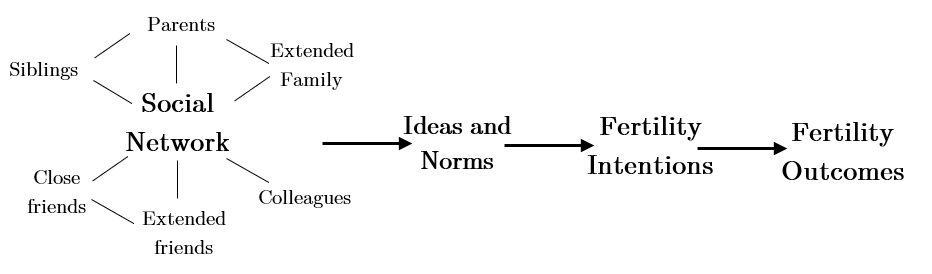
\includegraphics[width=0.95\linewidth]{figure/Figure_1} \caption{Social Network Processes.}\label{fig:figure1}
\end{figure}
Social contagion relies on explicit social networks and the strength of social networks. Granovetter (\protect\hyperlink{ref-granovetter1973}{1973}) state the strength of a tie between individuals to be a combination of time, emotional intimacy and reciprocal services. When measured, the size of social networks occur in a U-shaped curve over the life course; being low in young adulthood and peaking around 40 years of age, and then declining particularly after retirement ages (Micheli, \protect\hyperlink{ref-micheli2000}{2000}). The definition of a social network's size and composition depends on many variables, with the literature compounding age, marital status, employment status, education and gender as influencers (Diaz et al., \protect\hyperlink{ref-diaz2011}{2011}). Along with individual characteristics, social contagion moderates childbearing intentions and are included as an aggregate process in the neighbourhood-scale models. That is, first-order queen neighbourhood matrices based on contagion match the contagion effects of social networks.

\hypertarget{Data}{%
\chapter{Data}\label{Data}}

\hypertarget{geography}{%
\section{Geography}\label{geography}}

The boundary data is downloaded as a shapefile from the Office for National Statistics (ONS), with high-detailed polygon data. The MSOA polygons are irregular areal (lattice) data. In forming the neighbourhoods (MSOAs) of this dissertation, the merging of areas is undertaken by the ONS starting at the Output Area (OA). First, OAs are aggregated to Lower Super Output Areas (LSOAs), and then LSOAs to MSOAs. LSOAs are generated by merging typically 4 to 6 OAs based on 2011 census measures: population size, mutual proximity and social homogeneity. The MSOAs are considered to be theoretically sound neighbourhoods based on the three criteria above in forming a neighbourhood. The process of agglomeration is vital, as meaningful geographies must be theoretically robust in order to correctly understand fertility (Boyle et al., \protect\hyperlink{ref-boyle2007}{2007}). Mutual proximity results in a compact shape, and the specific homogeneity criteria is related to type of dwelling, that is, detached or semi-detached, and also the tenure, whether that be owner-occupied or socially rented (ONS, 2016). 2.1\% of MSOAs changed between the 2001 and 2011 versions, thereby creating reliable boundaries for an analysis of 2011 data. Figure 3.1 shows this process in the MSOA surrounding the University of Southampton, Highfield campus, with the final map showing the highlighted neighbourhood in the Local Authority of Southampton.
\begin{figure}
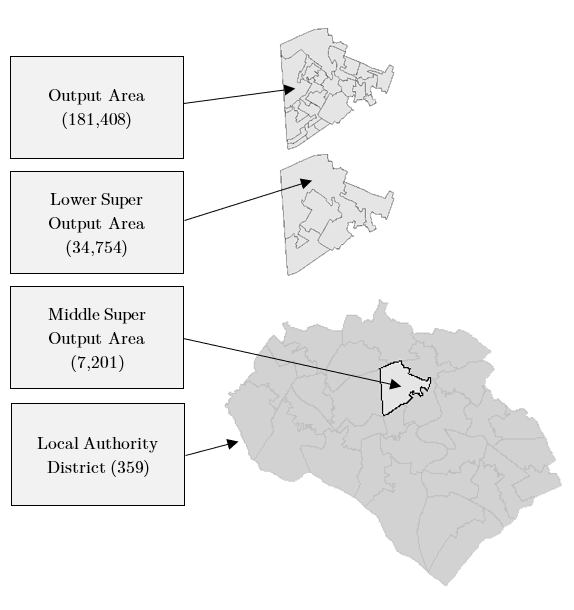
\includegraphics[width=0.8\linewidth]{figure/Figure_2} \caption{Process of aggregation in Southampton (England and Wales counts). Boundary data source: UK data service, own depiction.}\label{fig:figure2}
\end{figure}
Once created, the MSOAs of England and Wales number 7,201 MSOA. The polygons include water bodies, as well as some parts of the coast, therefore distorting the population density of certain coastal regions slightly. Despite minor limitations in the polygon data, the 2011 MSOA boundaries are well-suited to be compared, as the 2011 census was used to formulate the 2011 MSOA boundaries. However, cross-time comparisons of spatial dependence become more contentious due to large population changes from 2002 to 2018. The Isles of Scilly, forming one MSOA, are completely excluded from this dataset, being the only neighbourhood without a neighbour.

\hypertarget{birth-registration-and-mid-year-population-estimates}{%
\section{Birth registration and mid-year population estimates}\label{birth-registration-and-mid-year-population-estimates}}

Vital registration and mid-year population estimates are the sources used to calculate Age-Specific Fertility Rates (ASFRs) and TFR. Vital registration data collated by the ONS provides a count of births by age of the mother in \textasciitilde10-year age brackets, and recording the residence of the mother is published also by the ONS (and available publicly as LSOA location). There are three strata of mothers: those aged under 24, those aged 25 to 34, and those aged above 35. The vital registration data is not aligned with the population estimate data. The above three strata of women are taken in this methodology to relate to women aged 15 to 24, 25 to 34 and 35 to 44, therefore excluding women under 15 and over 44 from calculations. In 2011, 4.4\% of births in England and Wales were by mothers over the age of 45, and the exclusion is somewhat problematic, but reduces greater misspecification. The exclusion of young mothers is non-problematic, as births to girls under the age of 15 are fewer than 0.01\% of all births (ONS, 2018). Mid-year population estimates are the denominator of the ASFR and TFR calculations. The mid-year population estimates count male and female populations in 5-year age brackets, with an open-ended `85 plus' group. The data is organised by address (and available publicly as LSOA location). Permanent migrants are included in the former data source, yet, those who intend to remain in the UK less than 12 months are excluded from mid-year population estimates. There also some exclusions in the mid-year population estimates of students at their term-time addresses and armed forces, although the degree to which the two latter groups will influence fertility is considered low. Therefore, the two data sources do not match entirely, and is this is considered in noting the accuracy of the results. The calculations of ASFR and TFR, with caveats, are below, with a being the 10-year age brackets: 15 to 24, 25 to 34 and 35 to 44:

\[ ASFR=\left(\frac{b_a}{w_a}\right)\ 1000 \]
\[ TFR=5\ \ \sum A S F R \]
\begin{table}

\caption{\label{tab:unnamed-chunk-3}Summary of explanatory variables.}
\centering
\resizebox{\linewidth}{!}{
\begin{tabu} to \linewidth {>{\raggedright}X>{\raggedright}X>{\raggedright}X>{\raggedright}X}
\toprule
Variable & Description & Calculation & Source\\
\midrule
Education & The percentage of women aged 25-44 who have university-level education and above & Female population with a degree or higher25-44 / Total female population25-44 & Census 2011\\
Ethnicity & The percentage of women aged 15-44 who are Pakistani, Bangladeshi, or Black African (each ethnicity is a separate variable) & Female population of certain ethnicity15-44 / Total female population­15-44 & Census 2011\\
Income & Average net weekly income (£) & Unchanged & ONS, 2020\\
Population density & The number of people per 1km2 & Total population / Polygon size (km2) & Census 2011 \& Polygon file\\
Divorce & The percentage of the population aged 16 and above that are divorced & Total population divorced16+ / Total population16+ & Census 2011\\
\addlinespace
Social Support & The proportion of dwellings (excluding non-residential buildings) that are socially rented & Dwellings socially rented / Total dwellings & Census 2011\\
Non-religious & The percentage of the population who are non-religious & Total population Non-religious / Total population & Census 2011\\
\bottomrule
\multicolumn{4}{l}{\textsuperscript{} \makecell[l]{All variables are continuous while population density is translated to log form due \\ to outliers and large variance.}}\\
\end{tabu}}
\end{table}
To clarify the definitions of variables in Table 3.1, education is calculated only with women aged 25-44. This variable counts those who have a degree level or above, and calculates the proportion of this group in relation to the entire female population aged 25-44. The age 25 is used as it is assumed that women above the age of 25 have mostly completed education and the highest qualification level will not vary greatly thereafter. The ethnicity variables count women aged 15-44 to match the ASFR and TFR calculations used. Income is derived from ONS estimates of MSOA income levels. Net monthly income more accurately captures the spending ability of individuals and is therefore used as opposed to gross income. The population density variable is derived from the polygon data itself by calculating the size of each MSOA in R, and taking the mid-year population estimate as the denominator. Population density is also transformed as extreme values are present. The prevalence of divorce, as intended to be a contextual variable, measures the entire population aged 16 and above. The social support variable is calculated from census data which categorises three types of dwelling tenure. That is, `owned or shared ownership', `social rented' and `private rented or living rent free'. In doing so, rented from the council (Local Authority) directly as well as socially rented from other sources are combined. The `social rented' category is divided by the sum of all dwellings within the MSOA, excluding non-residential buildings. The non-religious variable is taken from the entire population of both men and women of all ages in order to show the contextual role of secularism. All of these variables are proportions except for income, and in the model-building process, all are multiplied by 100 to ease in the interpretation of the models.

\hypertarget{Methodology}{%
\chapter{Methodology}\label{Methodology}}

Spatial autocorrelation is Tobler's first law of geography, famously stated as: ``everything is related to everything else, but near things are more related than distant things''. In clarifying the terms of importance behind Tobler's first law, spatial autocorrelation relates to dependence, whereas spatial heterogeneity relates to spatial structure (Anselin, \protect\hyperlink{ref-anselin1988}{1988}). Spatial autocorrelation, and in turn diffusion, is measured separately from spatial heterogeneity. Despite the focus on spatial autocorrelation, models assessing spatial heterogeneity are relevant within fertility research. In explaining spatial variation in fertility, Jeronimo Muniz (\protect\hyperlink{ref-jeronimomuniz2006}{2006}) finds Geographically-Weighted Regression (GWR) to perform better when measuring adjusted R-squared value compared to spatial autocorrelation models. In a South Korean example, Jung et al. (\protect\hyperlink{ref-jung2019}{2019}) also find a GWR model to have a higher R-squared value than a spatial autoregressive model in the same setting, with GWR greatly reducing spatial autocorrelation in the residuals. Haque, Das, \& Patel (\protect\hyperlink{ref-haque2019}{2019}) model the 621 districts of India using a global autocorrelation model and GWR local model to explain spatial fertility differentials. The differences in model performance are small when considering the significance of the theoretical approach, as the driving force for model selection is the theory, rather than explicit performance statistics.

In terms of specific packages used within R to enable this research, the \texttt{spatialreg} package is used to calculate weight matrices as well as the spatial models. Other packages such as \texttt{tidyverse}, \texttt{rgeos}, \texttt{sf} and \texttt{rdgal} are also replied upon for data management. All of the code used to conduct the methodology and results are available on GitHub in the \href{www.github.com/ross-barker-soton.com}{`Dissertation' repository}.In checking the reproducibility of the code and data used within R, the neighbourhood matrices, weights matrices, Spatial Lag Model and Spatial Error model were also tested in GeoDa. A region identifier is also used to check that the variable data and map file are correctly aligned when applying the weights matrices. The spatial econometric work of Luc Anselin informs the models, with the application of such models to R aided by materials from a course led by Sebastian Klüsener. The sources of code within this methodology are also partly derived from Roger Bivand's (2019) analyses of spatial data as well as code published relating to Mark Burkey's spatial \href{http://spatial.burkeyacademy.com/}{Burkeyacademy}.

A ``specific-to-general'' approach Elhorst (\protect\hyperlink{ref-elhorst2014}{2014}) is followed in the model-building process, in the order: Ordinary-Least Squares (OLS), Spatial Lag (SAR) model, Spatial Error Model (SEM), Spatial Durbin Model (SDM) and Spatial Durbin Error Model (SDEM). The SAR, SER and SDM models are from Anselin (\protect\hyperlink{ref-anselin1988}{1988}), but the notation here is largely taken from Elhorst (\protect\hyperlink{ref-elhorst2014}{2014}). The specific-to-general approach allows for a gradual increase in model complication and allows for earlier models to be nested in the latter models. The model terms show the role of spatial autocorrelation from different sources. In differentiating between standard OLS and spatial models, Elhorst (2014, p.5) directly state the spatially explicit variables as being:
\begin{itemize}
\tightlist
\item
  Endogenous interaction effects in the dependent variable (Y)
  \begin{itemize}
  \tightlist
  \item
    Seen in the notation as \(\rho Wy\).
  \end{itemize}
\item
  Exogenous interaction effects among the independent variable (X)
  \begin{itemize}
  \tightlist
  \item
    Seen in the notation as \(WX\theta\).
  \end{itemize}
\item
  Interaction effects among the error terms (\(\varepsilon\))
  \begin{itemize}
  \tightlist
  \item
    Seen in the notation as \(u=\lambda Wu+\ \varepsilon\).
  \end{itemize}
\end{itemize}
The methods relating to spatial autocorrelation and the model-building process are split into five sections. First, the identification of neighbours (6.1) and the creation of a spatial weight's matrix (6.2) form the cornerstone of the spatial approach. Following the selection of the row-standardised weight's matrix, spatial analysis can be undertaken with spatial autocorrelation tests (6.3), namely Local and Global Moran's I (Moran, 1950). The following model building process is twofold. First, the spatial elements stated above are added to the base OLS (6.4) and model selection methodologies are used to test which model and associated autoregression parameter is of best-fit and methodologically sound (6.5).

\hypertarget{calculating-neighbour-and-weight-matrices}{%
\section{Calculating neighbour and weight matrices}\label{calculating-neighbour-and-weight-matrices}}

The matrix captures two dimensions of spatial information, adding values to cross-sectional dependence between observations similar to time measurement in time series analysis (Kondo, \protect\hyperlink{ref-kondo2016}{2016}). \texttt{nb} relates to an unedited neighbourhood matrix, and \(W\) is the spatial weights matrix calculated with the \texttt{nb} matrix, necessary in cross-sectional analysis. \texttt{nb} simply identifies neighbours within the shapefile, shown in Figure 4.1. For instance, the neighbourhood of Highfield towards the North of Southampton neighbours 6 other MSOAs. The simplicity of the queen contingency-based neighbourhood matrix is routed in the theory of social contagion. That is, direct neighbours influence one another, rather than large-scale processes. Any length or type of border is treated as a neighbouring region, thereby inferring queen-based measurement rather than rook. 0 is given to non-neighbouring nodes (and the diagonal) and 1 is given to neighbouring nodes. This results in symmetricity in the \texttt{nb} file. Additional neighbour-identifying processes are possible (K-nearest, Distance 5km, Distance 10km, 2nd-order queen, Rook) but fall outside the contagion context. The resulting \texttt{nb} of network size (N) of 7,200 unique areas contains 41,870 non-zero links, with the average number of links being 5.815.
\begin{figure}
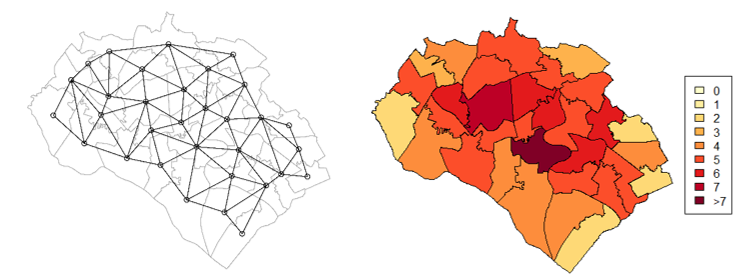
\includegraphics[width=0.95\linewidth]{figure/Figure_3} \caption{Neighbourhoods of Southampton.Note: links between Southampton and surrounding areas will be present; this figure is only for descriptive purposes. UK data service, own depiction.}\label{fig:figure3}
\end{figure}
By excluding of the Isles of Scilly from the dataset, there are no MSOAs without neighbours, yet, there are two isolated islands within the dataset: the Isle of Anglesey and the Isle of Wight. Due to the small-scale concept of neighbour, adding a link to the mainland is avoided. Scotland is the only land border lacking from this data, and the absence of neighbour-to-neighbour transmission over the Scottish-English border results in bias. Following the creation of neighbours, spatial dependence is added by transforming \texttt{nb} into \(W\). As with the \texttt{nb} matrix, \(W\) is of the dimension of the number of nodes in the network, \textbf{N.} The \(W\) matrix contains interactions which are of strength \(W_{ji}\). Here, \(i\) is a neighbour (MSOA) and \(j\) is a neighbour's neighbour. The combination of \texttt{W} and the endogenous spatial lag \(Y\), creates the spatial lag matrix \(Wy\), whereas the combination of the explanatory variables results in \(WX\), implying dependence. The following matrices are based on Anselin's work.
~

\({W\ }_{queen\left(Contiguity\right)}=\left(\begin{matrix}\begin{matrix}w_{11}&w_{12}&w_{13}&w_{14}\\w_{21}&w_{22}&w_{23}&w_{24}\\w_{31}&w_{32}&w_{33}&w_{34}\\w_{41}&w_{42}&w_{43}&w_{44}\\\end{matrix}\\\end{matrix}\right)\ \ \ \ \ {nb\ }_{queen\left(Contiguity\right)}=\left(\begin{matrix}\begin{matrix}0&1&0&0\\1&0&1&1\\0&1&0&1\\0&1&1&0\\\end{matrix}\\\end{matrix}\right)\ \ \ \ \)
~

The outcomes of autocorrelation and the hypotheses rejected/accepted depend on the neighbourhood and weights matrices chosen to varying degrees (Bivand, Pebesma, \& Gómez-Rubio, \protect\hyperlink{ref-bivand2013}{2013}). The \texttt{nb} calculation is more important than \(W\), as the method of \(W\) standardisation has relatively little effect on spatial regression results (Dormann et al., \protect\hyperlink{ref-dormann2007}{2007}; LeSage \& Pace, \protect\hyperlink{ref-lesage2014}{2014}). The standardisation and application of spatial weights matrices are either p-order, binary, contingency matrices, inverse distance, q-nearest neighbour, or block diagonal (Elhorst, \protect\hyperlink{ref-elhorst2014}{2014}). Binary coding is preferred when little is known about the spatial processes ongoing (Bavaud, \protect\hyperlink{ref-bavaud1998}{1998}), whereby neighbouring nodes are of equal influence regardless of the number of neighbours. The row-standardised approach assumes that the influence of a neighbour is spread between neighbours, therefore, no areas are heavily overpowered in influence. The row-standardisation approach leads to asymmetry in the matrix as by normalising \(W\), whereas the \texttt{nb} matrix is symmetric. Row normalisation equalises the impact of each MSOA, with no neighbourhood being more powerful than another (Elhorst, \protect\hyperlink{ref-elhorst2014}{2014}). In doing so, the sum of each row is 1, and the sum of all weights is 7200 (\textbf{N}).
~

\(W_{row-standardised}=\left(\begin{matrix}\begin{matrix}0&0.5&0.5&0\\0.33&0&0.33&0.33\\0.33&0.33&0&0.33\\0&0.5&0.5&0\\\end{matrix}\\\end{matrix}\right)\ \)
~

\(Wy=\left(\begin{matrix}\begin{matrix}0&0.5&0.5&0\\0.33&0&0.33&0.33\\0.33&0.33&0&0.33\\0&0.5&0.5&0\\\end{matrix}\\\end{matrix}\right)\ \left(\begin{matrix}\begin{matrix}y_1\\y_2\\y_3\\y_4\\\end{matrix}\\\end{matrix}\right)\ =\ \left(\begin{matrix}\begin{matrix}{1/2y}_2\ +\ {1/2y}_3\\{1/3y}_1\ +\ {{1/3y}_3\ +\ 1/3y}_4\\{1/3y}_1\ +\ {1/3y}_2+{1/3y}_3\\{1/2y}_2\ +\ {1/2y}_3\\\end{matrix}\\\end{matrix}\right)\ \)
~

\hypertarget{spatial-autocorrelation-tests}{%
\section{Spatial autocorrelation tests}\label{spatial-autocorrelation-tests}}

Following the finalisation of first-order contingency weights, both local and global tests of Moran's I are used to test for the existence of spatial dependence and illustrate dependence. The resulting values range from -1 to +1, with 0 showing no autocorrelation. -1 suggests negative spatial autocorrelation with neighbours showing opposing outcomes, whereas a positive Moran's I value shows positive association, as expected though social contagion processes. Local Indicators of Spatial Autocorrelation (LISA, Anselin, \protect\hyperlink{ref-anselin1995}{1995}) diagnose specific units exhibiting spatial dependence, and the LISA values sum to equal the global Moran's I statistic (Darmofal, \protect\hyperlink{ref-darmofal2015}{2015}). The LISA values are accompanied by significance p-values, showing areas of high-high, low-high, high-low, and low-low spatial dependence. The Moran scatter plot will display these alternative outcomes.

Moran's I is based on the spatial lag of the variable of choice, as a ratio of \(Y\) and its spatial lag (Bivand et al., \protect\hyperlink{ref-bivand2013}{2013}). In the equation, as shown and explained by Bivand et al. (\protect\hyperlink{ref-bivand2013}{2013}), \(W_{i}\) is the \(i\)th observation, and \(\bar{y}\) is the mean of the variable of interest. This is seen in the Moran scatter plot as the centre. \(W_{ij}\) is again the link between area \(i\) and its neighbour \(j\). Deviance from the mean is therefore associated with assumed spatial dependence. As Local Moran's I relates to individual observations (\(i\))and sums to the Global value, the same assumptions as above are used. The greatest difference is testing for the divergence of one particular area from the global mean. The Moran's I calculation is also used as a diagnostic tool for OLS residuals, specified as unfocused diagnostics, and generally identifying spatial dependence (Darmofal, \protect\hyperlink{ref-darmofal2015}{2015}). The Moran's I statistic is not useful for the comparison of spatial autoregressive models, as including a spatial element will undoubtably lead to a reduction in residual spatial dependence.

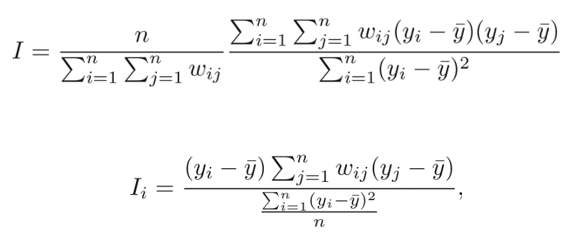
\includegraphics[width=0.65\linewidth]{figure/Equations}

\hypertarget{model-equations}{%
\section{Model equations}\label{model-equations}}

OLS is used as a benchmark in model comparison and as a starting point for the incorporation of spatially explicit variables. In selecting and analysing the results of a spatial model, either (or both) global and local effects are included, dependent on the type of spatial effect. Endogenous interaction cannot lead to just local spillovers, as a change in one neighbourhood can lead to global changes, with local spillover relating clearly to social contagion (LeSage \& Pace, \protect\hyperlink{ref-lesage2014}{2014}). For example, the autocorrelation between two neighbourhoods in Cornwall will be felt, even to a very minuscule amount, in Southampton, a feature known as simultaneous feedback (LeSage, \protect\hyperlink{ref-lesage2008}{2008}). Local models restrict effects of autocorrelation to direct neighbours, and result in no feedback throughout the entire model, occurring in the Spatial Error Model.\\
\hspace*{0.333em}

\(y=\beta_0+X\beta+\ \varepsilon\) ~\\
\hspace*{0.333em}

The model explanations and notations are a mixture of sources, largely from Elhorst (\protect\hyperlink{ref-elhorst2014}{2014}) and Anselin (\protect\hyperlink{ref-anselin1988}{1988}). First, Ordinal Least-Squares Regression (OLS) is presented. As common throughout all models, \(X\) is a matrix of the explanatory variables and \(\beta\) is the respective vector, representing the linear slope inferred by the explanatory variables. \(\varepsilon\) is the independent error term prevalent throughout all models.\\
\hspace*{0.333em}

\(y\ =\rho Wy+X\beta+\ \varepsilon\)\\
\hspace*{0.333em}

Second, the Spatial Lag (SAR) model hosts one addition to OLS; \(\rho Wy\), which adds spatial autoregression of the \(Y\) variable. The \(\rho\) is the strength (coefficient) of the endogenous, spatially lagged dependent variable \(Wy\), with this model therefore often termed the simultaneous autoregressive model. \(W\) is the spatial weight matrix. The SAR model has been criticised for omitting spatially dependent variables, \(WX\), which could lead to \(Wy\) being significant, when this is in fact not the case (Corrado \& Fingleton, \protect\hyperlink{ref-corrado2012}{2012}), an issue overcome in the Spatial Durbin Model. In essence, the SAR model assumes directional spatial effect from one area to its neighbour, closely supported by the theoretical background of this dissertation.\\
\hspace*{0.333em}

\(y\ =X\beta+u,\ u=\lambda Wu+\ \varepsilon\)\\
\hspace*{0.333em}

Third, the Spatial Error Model (SEM) includes spatial autoregression in the disturbance process \(varepsilon\ \), rather than in the dependent or explanatory variables, diverging from the theoretical standpoint of this dissertation. The new addition to this variable is \(Wu\), which is the interaction effect in the disturbance term. This model is similar to the OLS model in lacking the required analysis of direct, indirect and total impacts, and can be interpreted similarly (Elhorst, \protect\hyperlink{ref-elhorst2014}{2014}). The total impacts are calculated by Monte Carlo simulation as described by (LeSage \& Pace, \protect\hyperlink{ref-lesage2010}{2010}). The spatial autoregressive coefficient is shown in model output as \(lambda\ \). In sum, the spatial autocorrelation in the SEM is seen as a nuisance that is not linked to a specific cause, whereas SAR directly incorporates y (Harris, \protect\hyperlink{ref-harris2009}{2009}). The model is therefore not very spatial in nature, dealing with clustering. This model is therefore not expected to be theoretically justifiable, but will aid in model comparison.\\
\hspace*{0.333em}

\(y\ =pWy+X\beta+WX\theta+\ \varepsilon\)\\
\hspace*{0.333em}

Fourth, the Spatial Durbin Model (SDM) builds upon the SAR model through the inclusion of spatial autocorrelation in the explanatory variables. This in turn adds a local aggregation component to the SAR model (Dormann et al., \protect\hyperlink{ref-dormann2007}{2007}). The addition to this model is \(WX\theta+\ \), which describes the coefficients of the spatially lagged explanatory variables \(WX\). \(\theta+\) functions similarly to \(\beta\), but represents unknown parameters. By including both \(WX\) and \(Wy\) in the model, the omitted variable problem that boosts the endogenous spatial lag significance is mitigated as well as allowing exogenous variation (Corrado \& Fingleton, \protect\hyperlink{ref-corrado2012}{2012}). Therefore, a more methodologically sound and accountable model is produced, although interpretation is less intuitive. In comparing SDM results to the SAR model, effects are often greater in the SDM model due to the exogenous interaction (Golgher \& Voss, \protect\hyperlink{ref-golgher2016}{2016}). Both the SAR and SDM model contain lagged \(y\), and therefore cannot treat the coefficients of the summary model as marginal effects, but instead calculate direct (DE), indirect (IE) and total marginal effects (TE) (Bivand et al., \protect\hyperlink{ref-bivand2013}{2013}).\\
\hspace*{0.333em}

\(y\ =X\beta+Wx\theta+\ u,\ u=\lambda Wu+\ \varepsilon\)\\
\hspace*{0.333em}

Fifth, the Spatial Durbin Error Model (SDEM) adds lagged \(X\) variables to the SEM, similarly to SDM gaining lagged \(y\). This model therefore does not include the y variable as an explanatory variable within the model. Due to the catch-all characteristic that arises from the inclusion of error interaction, the interpretation of the model is far from intuitive, although the comparative strength of the model is expected to be high.

\hypertarget{robustness-checks}{%
\section{Robustness checks}\label{robustness-checks}}

Model specification is largely derived from tests on the OLS model. The analytical approach within this dissertation expects both diffusion and the clustering of similar behaviours, therefore, both the SAR model and the SEM are expected to be robust. Questions arise as to whether the model should be further complicated to the SDM in order to account for potentially significant exogenous effects. LeSage (\protect\hyperlink{ref-lesage2014a}{2014}) argue that only the SDM and SDEM models should be considered in spatial modelling, as they capture the effects of the SAR model and SEM, while accounting for conflicting spatial processes that would arise bias if omitted. The diagnostic approach uses Larange Multiplier (LM) tests to navigate model specification.

First, LM Tests based on the OLS results are undertaken, whereby the weights matrix is incorporated into the test to decide whether the SAR model and/or SEM is justifiable (Anselin, Bera, Florax, \& Yoon, \protect\hyperlink{ref-anselin1996}{1996}). These tests are written as LMerr and LMlag. Whether LMerr or LMlag is significant shows which model should be continued and built upon further, in this case either in a SDM or SDEM. The focussed diagnostics above identify either spatial lag or spatial error dependence, but a standard LR test cannot be used as one could element may detect the other (Darmofal, \protect\hyperlink{ref-darmofal2015}{2015}). Therefore, robust LM diagnostic tests developed by Bera \& Yoon (\protect\hyperlink{ref-bera1993}{1993}) are used that account for false positives, named RLMerr and RLMlag that are robust to the presence of the other type of autocorrelation. Once completed, the Akaike Information Criterion (AIC, Akaike, \protect\hyperlink{ref-akaike1974}{1974}) is used to compare models, as the adjusted R-squared value is incomparable with the autoregressive models used.

\hypertarget{results}{%
\chapter{Results}\label{results}}

The results of the data analysis and models are presented here in four sections. First, univariate and bivariate statistical analysis is undertaken (7.1), focussing on the spatial, unmodelled description of the data. Second, Global Moran's I is used to test whether spatial autocorrelation exists in TFR in England and Wales (7.2); all variables will be tested in this manner. Local Moran's I is used to display clustering of neighbourhoods that exhibit spatial dependence. Third, an OLS model will be built with all the variables deemed significant based on the literature and theoretical approach (7.3), with stepwise addition of the variables. This section will display how Global Moran's I changes with the addition of variables and whether such variables may account for what is assumed to be spatial autocorrelation led by social networks. The fourth and final section compares the four spatial models in exploring and interpreting small-scale fertility determinants (7.4).

\hypertarget{descriptive-results}{%
\section{Descriptive results}\label{descriptive-results}}

\hypertarget{total-fertility-rate}{%
\subsection{Total Fertility Rate}\label{total-fertility-rate}}

The TFR of England and Wales was 1.93 in 2011, with the values of MSOA TFR varying from 0.304 to 4.584, with a mean of 1.961. England and Wales has relatively high TFR in the European context, following a decline from 1.93 in 2011 to 1.65 in 2019 (ONS, 2020). England and Wales has never experienced lowest-low fertility of below 1.3 (H. Kohler et al., \protect\hyperlink{ref-kohler2002b}{2002}), but 342 of the 7,200 MSOAs are within this classification in 2011. Moreover, 2,750 MSOAs host TFR above replacement level (2.1). Vast spatial differentiation is present, with local context seeming to influence fertility greatly. ASFRs also vary similarly. The mean value of ASFR ages 15-24 is 49.1 births per 1,000 women, with a height of 188 births per 1,000 women. The mean value of ASFR ages 25-34 is 110 births per 1,000 women, with a height of 215 births per 1,000 women. The mean fertility rate of the women aged 35-44 is 36 births per 1,000 women, with a height of 123 births per 1,000 women. Figure 5.1 shows the temporal change in TFR distribution of MSOAs in 2002, 2011 and 2018, coloured by the TFR value of each neighbourhood in 2011, being low (\textless1.3), middle (1.3-2.1) and high (\textgreater2.1). Throughout the time period, there appears to be little difference in the location of lowest-low fertility within England and Wales, with the distribution remaining normal.
\begin{figure}
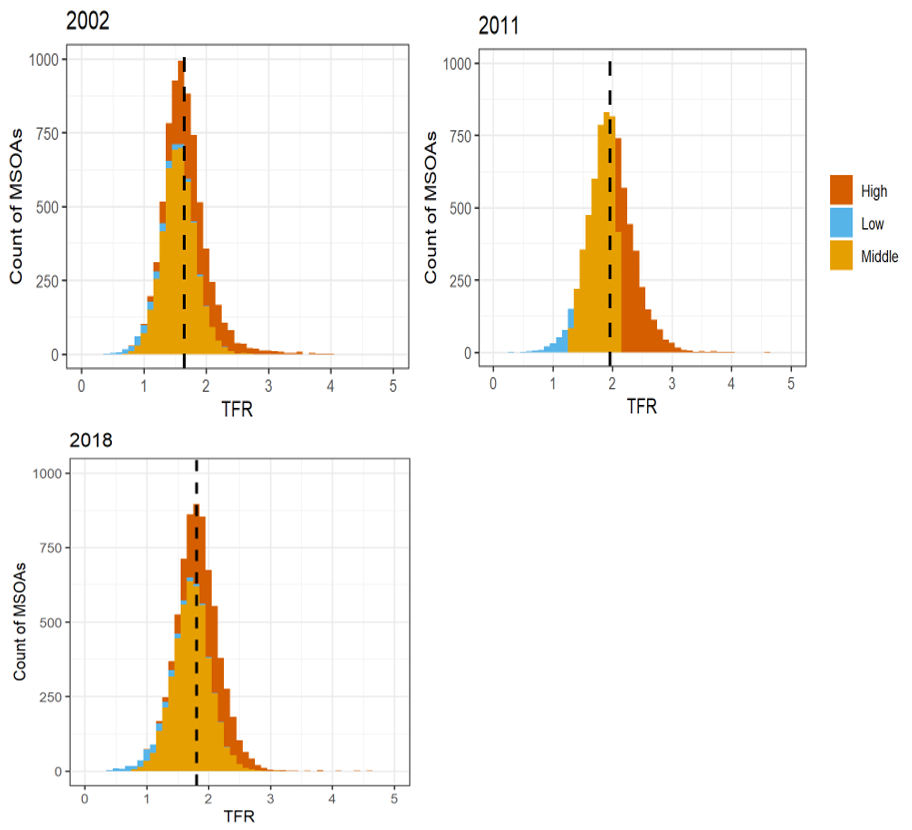
\includegraphics[width=0.95\linewidth]{figure/Figure_4} \caption{MSOA TFR Histogram. Note: Low (<1.3), middle (1.3-2.1) and high (>2.1) TFR categorisation taken from 2011 levels. Source: ONS, own calculations.}\label{fig:figure4}
\end{figure}
\begin{figure}
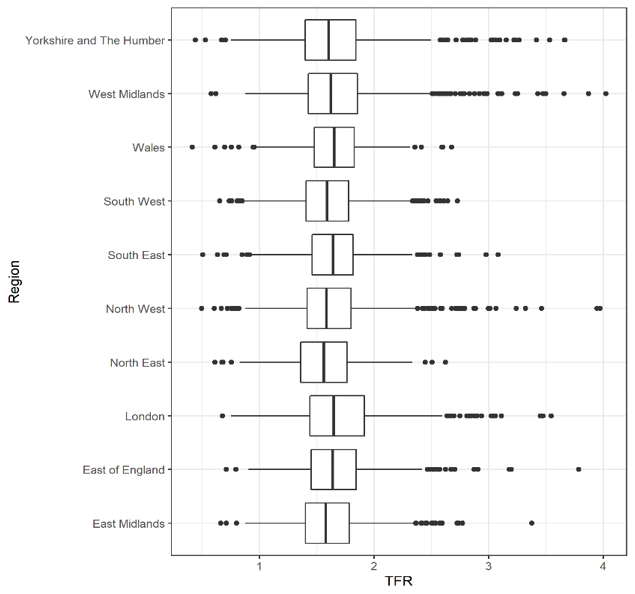
\includegraphics[width=0.95\linewidth]{figure/Figure_5a} \caption{Regional TFR 2002. Source: ONS, own calculations.}\label{fig:figure5a}
\end{figure}
\begin{figure}
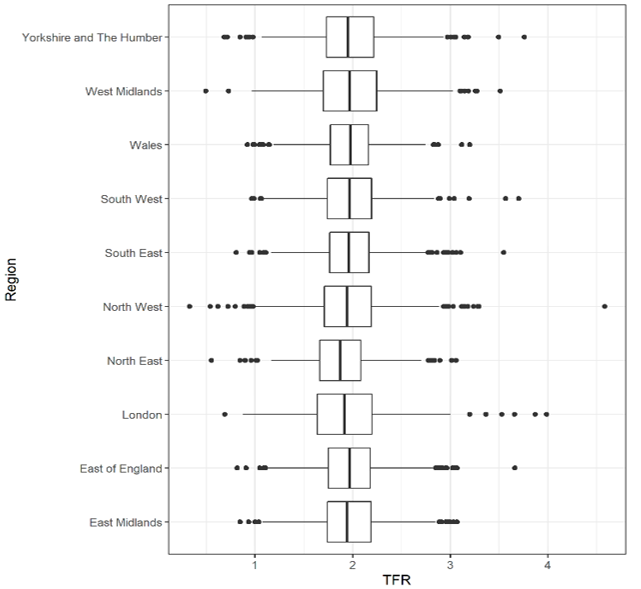
\includegraphics[width=0.95\linewidth]{figure/Figure_5b} \caption{Regional TFR 2011. Source: ONS, own calculations.}\label{fig:figure5b}
\end{figure}
\begin{figure}
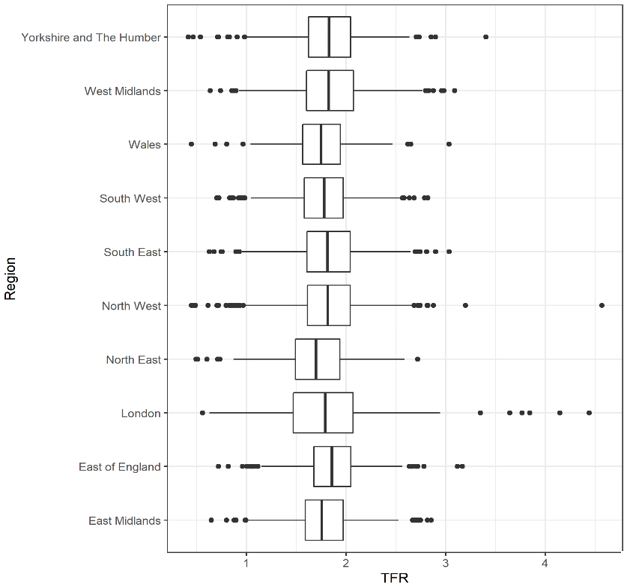
\includegraphics[width=0.95\linewidth]{figure/Figure_5c} \caption{Regional TFR 2018. Source: ONS, own calculations.}\label{fig:figure5c}
\end{figure}
The regional differences in TFR are not greatly pronounced. The temporal changes are, however, as the rise in TFR to 2011 shows all regions approaching mean TFR of 2, whereas in 2002, no regions had an upper quartile within this range. 2018 data shows a return to levels similar to 2002, with regions hosting slightly lower TFR than in 2011 and retaining regional differences. The region showing the greatest variance is London at each time point, as well as continuously hosting outliers with very high TFR above 3. At each time, an MSOA with extremely low and extremely high TFR is present in each region, with no evidence of fertility behaviour convergence to the national average. In sum, there are clear local differences that persist throughout England and Wales, and no evidence in support of regional convergence.

\hypertarget{explanatory-variables}{%
\subsection{Explanatory Variables}\label{explanatory-variables}}
\begin{table}

\caption{\label{tab:table2}Descriptive statistics of explanatory variables, 2011.}
\centering
\begin{tabu} to \linewidth {>{\raggedright}X>{\raggedright}X>{\raggedright}X}
\toprule
Variable & Overall...n..7200. & Global.Moran.s.I\\
\midrule
Education &  & 0.66266***\\
Mean (SD) & 0.292 (0.124) & \\
Range & 0.051 - 0.803 & \\
Pakistani &  & 0.62856***\\
Mean (SD) & 0.020 (0.061) & \\
\addlinespace
Range & 0.000-0.794 & \\
Bangladeshi &  & 0.67522***\\
Mean (SD) & 0.008 (0.029) & \\
Range & 0.000 – 0.743 & \\
Black African &  & 0.77529***\\
\addlinespace
Mean (SD) & 0.020 (0.028) & \\
Range & 0.000 – 0.431 & \\
Net Weekly Income (£) &  & 0.66819***\\
Mean (SD) & 731.360 (190.061) & \\
Range & 300.000 - 1730.000 & \\
\addlinespace
Population Density (non-logarithmic) &  & 0.73903***\\
Mean (SD) & 3157.226 (3396.420) & \\
Range & 5.672 - 24715.644 & \\
Social Housing &  & 0.34774***\\
Mean (SD) & 0.174 (0.132) & \\
\addlinespace
Range & 0.002 - 0.794 & \\
Divorce &  & 0.44204***\\
Mean (SD) & 0.091 (0.020) & \\
Range & 0.014 - 0.184 & \\
Non-Religious &  & 0.69668***\\
\addlinespace
Mean (SD) & 0.252 (0.074) & \\
Range & 0.018 - 0.576 & \\
\bottomrule
\multicolumn{3}{l}{\textsuperscript{} The spatial autocorrelation graphs are in appendix 1.}\\
\multicolumn{3}{l}{Source: ONS, own calculations.}\\
\end{tabu}
\end{table}
Table 5.1 shows the explanatory variables used in the 2011 models. These varaibles coded in percentage terms mostly show large variance, with the proportion of the adult population who are divorced showing the smallest range. This is accompanied by a relatively low mean divorced proportion of 9.1\%. University-level education has a very wide range and mean of 29.2\%. The Global Moran's I values are significant at the 0.001\% level and positive for each variable, showing that all are positively spatially dependent, similarly to TFR. Expectedly, spatial autocorrelation is very strong in the population density variable. The Black African population is similarly highly spatially autocorrelated, and social housing is the explanatory variable showing the lowest Moran's I value.
\begin{figure}
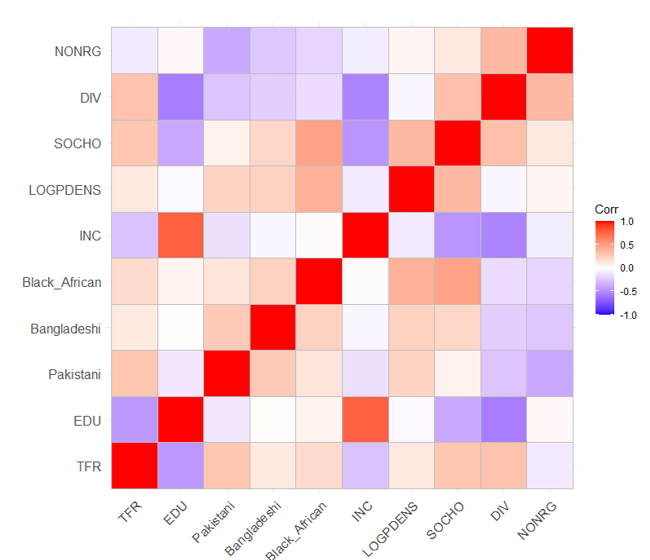
\includegraphics[width=0.95\linewidth]{figure/Figure_6} \caption{Bivariate Correlation. Source: ONS, own calculations.}\label{fig:figure6}
\end{figure}
A correlation matrix is shown in Figure 5.5, with the highest correlations occurring in the relationships that include income and education. Income appears to be a leading variable showing very negative association with social housing and the divorce variable. Divorce is also very negatively associated with education. Only Bangladeshi-Education and Black African-Income associations are non-significant. TFR-specific bivariate associations are also displayed in figure 5.6 on the following page. University-level education has a clear negative relationship with TFR. In contrast, the Pakistani, Bangladeshi and Black African variables are clearly positively associated with TFR. Income appears to be negatively associated with TFR, however, once reaching roughly £500 net income per week, the effect of income appears to flatline. Population density shows a slightly inverted U-shaped curve; TFR increases gradually to a population density around 5,000 residents/km2, roughly comparable to a town or city centre. Then, areas of very high population density have increasingly low TFR. The argument within the literature that low population density is associated with low TFR may not hold within the UK context, as it appears that very rural areas host some of the lowest fertility, alongside highly urban city centre neighbourhoods. Socially rented dwellings, similarly to the ethnicity results, show a clear increase in TFR as the proportion of socially rented homes increase. As divorce prevalence in a neighbourhood increases, as does TFR. The non-religious variable is less clear, as the influence is felt at the lowest and highest values of non-religious proportions, and not in the central, most frequent counts. Therefore, the role of non-religious proportions seems to be one of the weakest variables included.
\begin{figure}
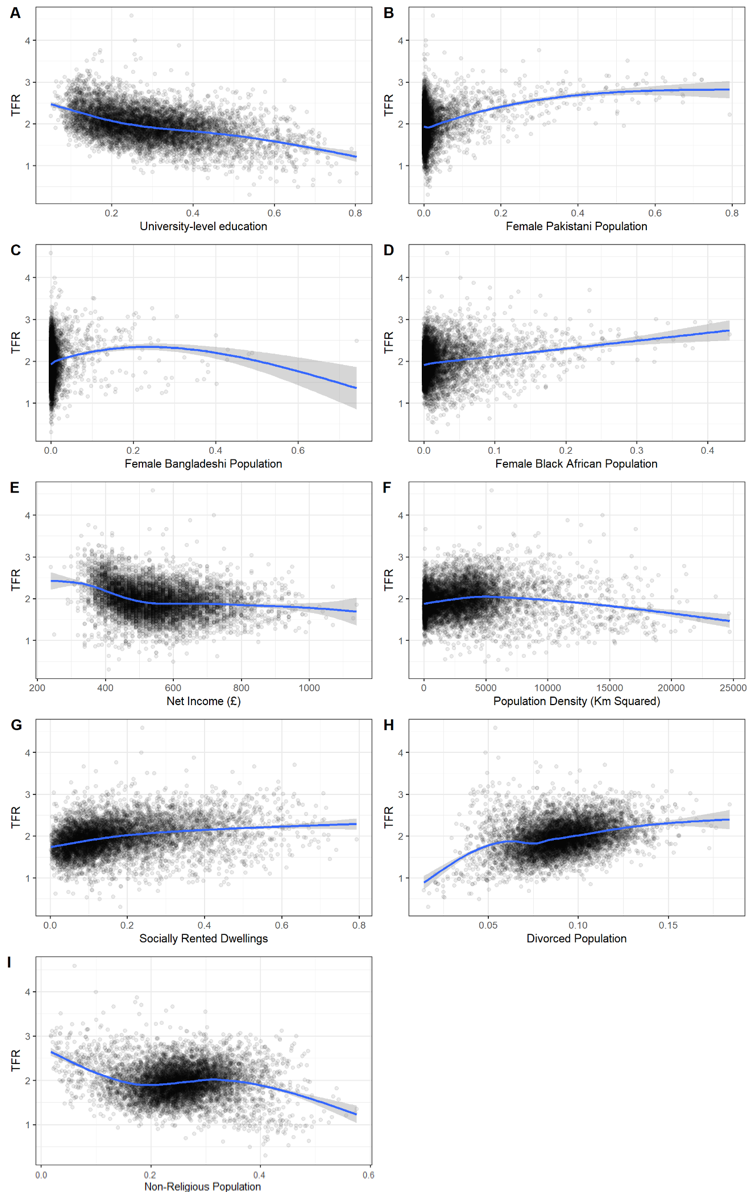
\includegraphics[width=0.95\linewidth]{figure/Figure_7} \caption{Bivariate association with line of best fit. N=7200. Source: ONS, own calculations.}\label{fig:figure7}
\end{figure}
\hypertarget{global-and-local-morans-i}{%
\section{Global and Local Moran's I}\label{global-and-local-morans-i}}
\begin{figure}
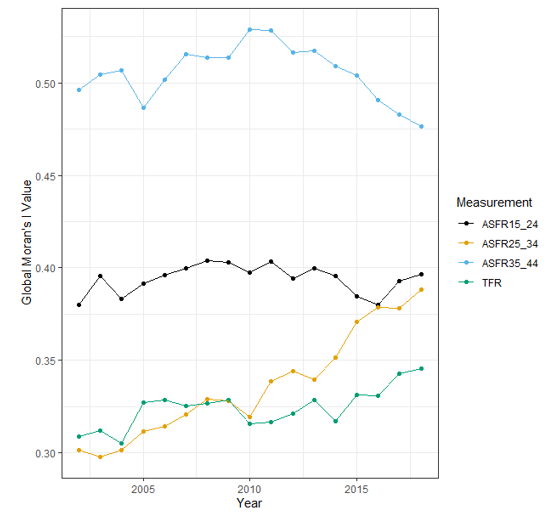
\includegraphics[width=0.95\linewidth]{figure/Figure_8} \caption{Global Moran's I - Fertility variables. Source: ONS, own calculations.}\label{fig:figure8}
\end{figure}
This section addresses the first research question: is there spatial autocorrelation in fertility outcomes, and if so, has this been weakening or strengthening over time (from 2002-2018)? Figure 5.7 shows global Moran's I calculated for ASFRs and TFR from 2002 to 2018. Throughout the roughly two decades, the spatial autocorrelation of the separate ASFRs show three separate trends. All three ASFRs are highly significantly spatially autocorrelated, however, the increase in TFR spatial dependence may be led by an uptake in the spatial dependence of fertility of women aged 25 to 34. This group of women hosted the lowest Moran's I value in 2002, far below that of women aged 15 to 24. However, the gap between these two measures is near-eliminated by 2018. The ASFR of women aged 35 to 44 remains the highest throughout the time period but shows a gradual and persistent decline from 2013 to 2018. Only the spatial autocorrelation value of women aged 15 to 24 has remained stable, while the two remaining groups showed marked changed beginning roughly in 2014. The answer to the question is therefore that the differences in spatial autocorrelation between ASFRs has weakened, however, the spatial dependence of TFR has strengthened.
\begin{figure}
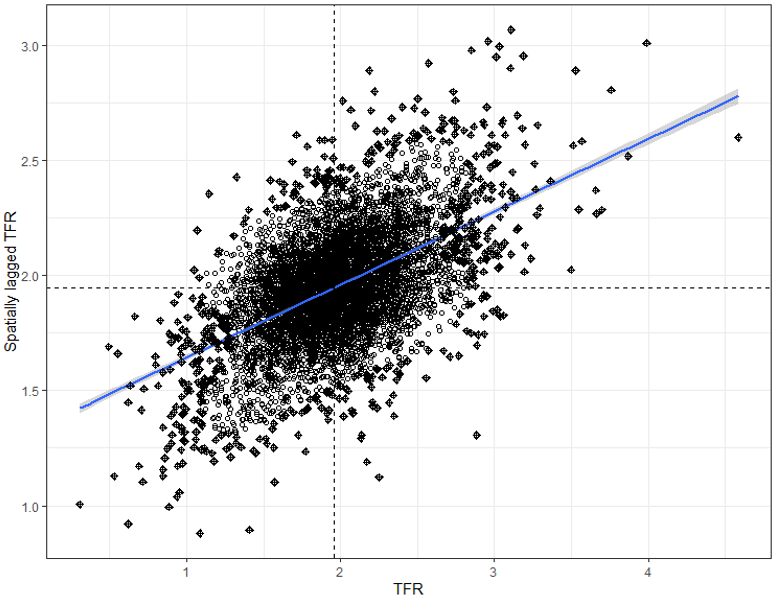
\includegraphics[width=0.95\linewidth]{figure/Figure_9} \caption{Spatially lagged TFR versus TFR. Source: ONS, own calculations.}\label{fig:figure9}
\end{figure}
The Global Moran's I value of TFR in 2011 provides a value of 0.3167, significant at the 0.001\% level. This background of this value is shown in Figure 5.8, with TFR plotted against spatially lagged TFR. The quadrants of the graph display high-high (top right) and low-low (bottom left) relationships with significance increasing the further from the centre (mean). Low-high values are situated in the top left, and high-low values in the bottom right, showing negative autocorrelation, although few are significant at the 5\% level, as seen in the oncoming maps. The scatterplot shows positive autocorrelation, with a general sign that the higher TFR of area \(i\), the higher the TFR of \(i\)'s neighbour, \(j\), and vice versa. The pattern in Local Indicators of Spatial Autocorrelation (LISA) shows substantive variability even within towns, relationships overlooked by regional and national analyses. The LISA values are mapped on the three following pages, whereby the clustering of spatial dependence can be seen. The example of London contains patterns seen nationally, with low-low dependence in the highly urbanised, very highly populated areas, and high-high significance in areas with large amounts of high-fertility ethnic minorities. Significant clustering is rarely isolated between two neighbourhoods, but rather a collection of spatially dependent MSOAs. Examples of the clustering phenomenon are in MSOAs surrounding Winchester in the South East of England, and a corridor of low-low dependence meandering down the centre of Devon and Cornwall, linked to Ilfracombe.
\begin{figure}
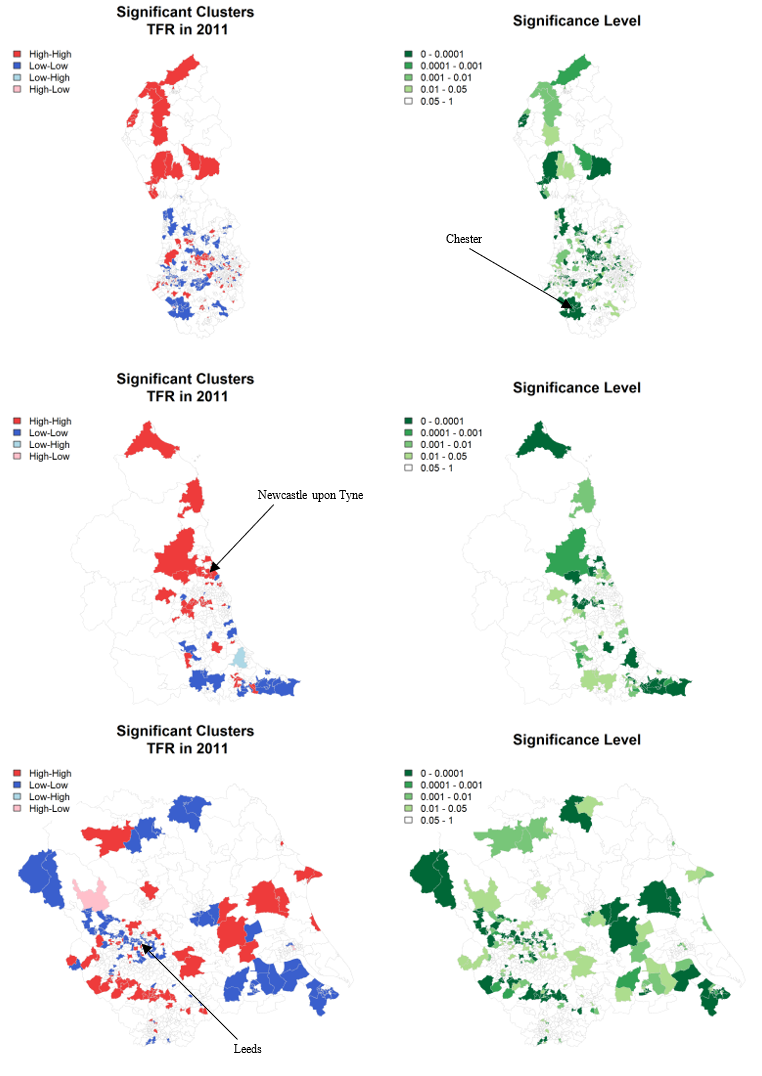
\includegraphics[width=0.95\linewidth]{figure/Figure_10} \caption{Local Moran's I values. North West England (Top), North East England (Middle), Yorkshire and the Humber (Bottom). Source: ONS, UK data service, own calculations}\label{fig:figure10}
\end{figure}
\begin{figure}
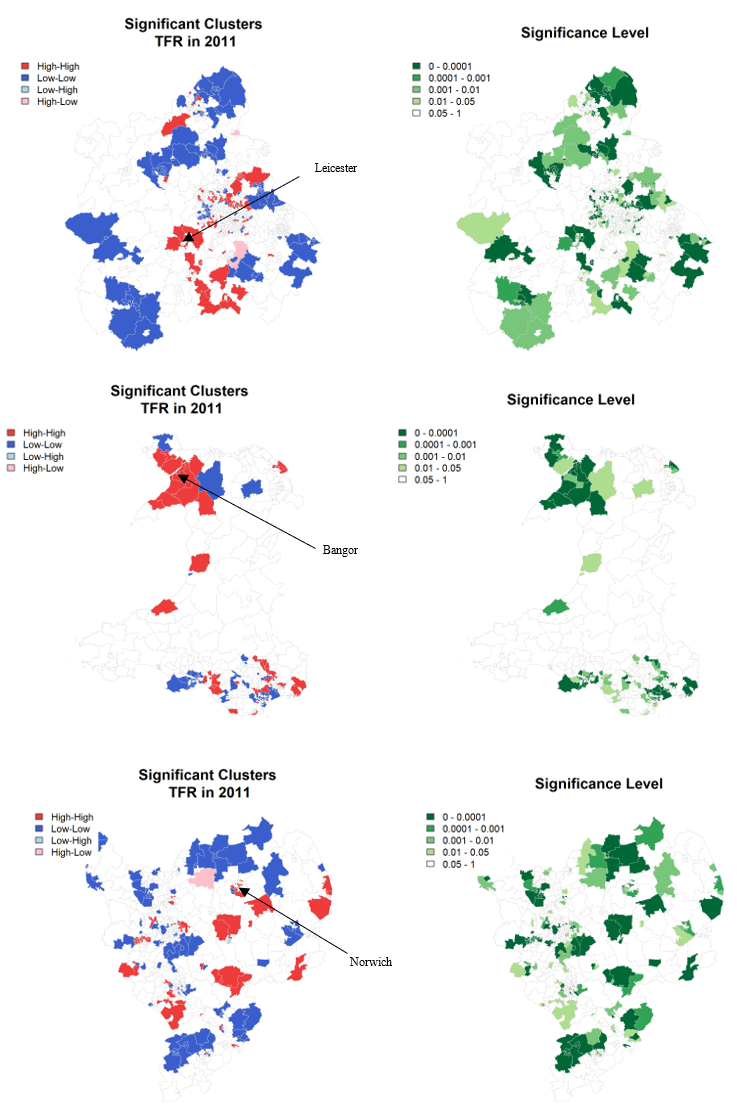
\includegraphics[width=0.95\linewidth]{figure/Figure_11} \caption{Local Moran's I values. East Midlands (top), Wales (middle), East of England (bottom). Source: ONS, UK data service, own calculations}\label{fig:figure11}
\end{figure}
\begin{figure}
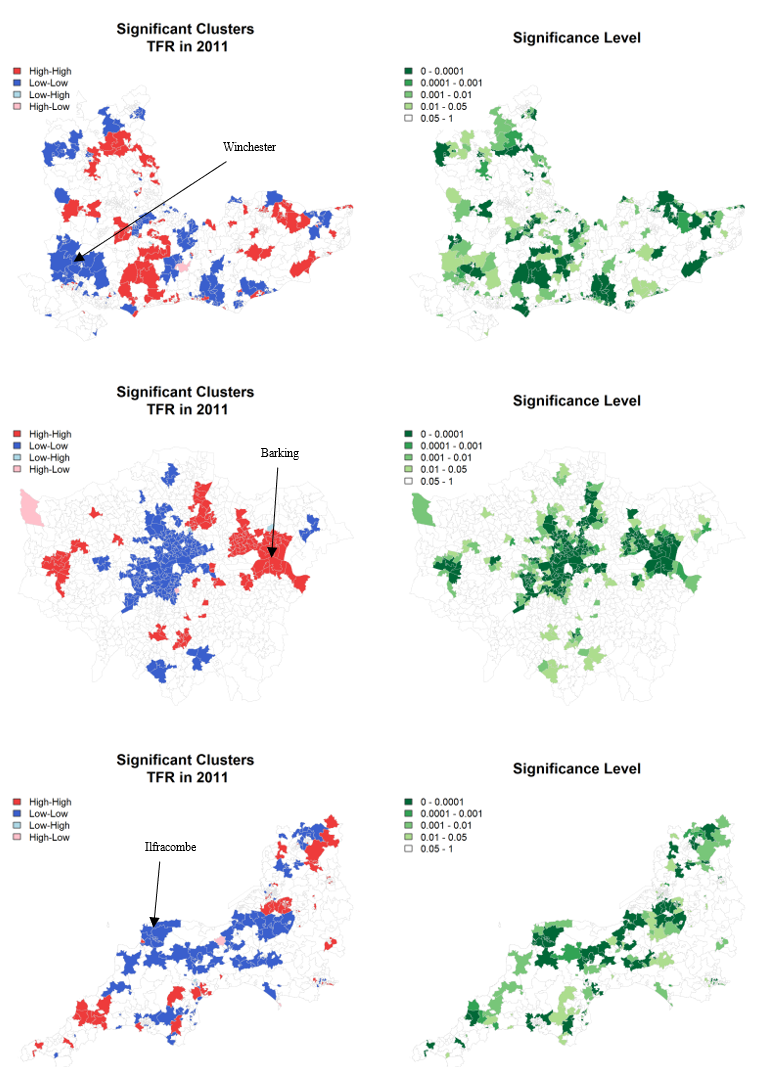
\includegraphics[width=0.95\linewidth]{figure/Figure_12} \caption{Local Moran's I values. South East England (top), London (middle), South West England (bottom). Source: ONS, UK data service, own calculations}\label{fig:figure12}
\end{figure}
\begin{landscape}\begingroup\fontsize{8}{10}\selectfont
\begin{longtabu} to \linewidth {>{\raggedright}X>{\raggedright}X>{\raggedright}X>{\raggedright}X>{\raggedright}X>{\raggedright}X>{\raggedright}X>{\raggedright}X>{\raggedright}X>{\raggedright}X}
\caption{\label{tab:table3}OLS Results (discussed on the following page).}\\
\toprule
Variable & Model 1 & Model 2 & Model 3 & Model 4 & Model 5 & Model 6 & Model 7 & Model 8 & Model 9\\
\midrule
Intercept & 2.366*** & 2.312*** & 2.31*** & 2.29*** & 1.996*** & 2.027*** & 1.893*** & 1.098*** & 1.097\\
 & (-0.01) & (-0.01) & (-0.01) & (-0.01) & (-0.019) & (-0.028) & (-0.03) & (-0.041) & (-0.041)\\
Education & -1.386*** & -1.308*** & -1.314*** & -1.353*** & -2.01*** & -2.008*** & -1.957*** & -1.595*** & -1.6\\
 & (-0.033) & (-0.031) & (-0.031) & (-0.031) & (-0.049) & (-0.047) & (-0.048) & (-0.047) & (-0.049)\\
Pakistani &  & 1.592*** & 1.51*** & 1.407*** & 1.474*** & 1.489*** & 1.598*** & 2.147*** & 2.152\\
\addlinespace
 &  & (-0.063) & (-0.066) & (-0.065) & (-0.063) & (-0.064) & (-0.064) & (-0.065) & (-0.069)\\
Bangladeshi &  &  & 0.617*** & 0.087 & 0.222 & 0.246' & 0.066 & 0.802*** & 0.809\\
 &  &  & (-0.141) & (-0.141) & (-0.137) & (-0.139) & (-0.138) & (-0.135) & (-0.136)\\
Black African &  &  &  & 1.916*** & 1.951*** & 2.011*** & 1.369*** & 1.991*** & 2\\
 &  &  &  & (-0.104) & (-0.102) & (-0.109) & (-0.122) & (-0.119) & (-0.122)\\
\addlinespace
Income &  &  &  &  & 0.001*** & 0.001*** & 0.001*** & 0.001*** & 0.001\\
 &  &  &  &  & (-0.00005) & (-0.00005) & (-0.00005) & (-0.00005) & (-0.00003)\\
Population Density (log) &  &  &  &  &  & -0.004 & -0.011*** & -0.012*** & -0.012\\
 &  &  &  &  &  & -(0.003) & (-0.003) & (-0.003) & (-0.0026)\\
Social Housing &  &  &  &  &  &  & 0.443*** & 0.195*** & 0.193\\
\addlinespace
 &  &  &  &  &  &  & (-0.039) & (-0.038) & (-0.038)\\
Divorce &  &  &  &  &  &  &  & 6.599*** & 6.576\\
 &  &  &  &  &  &  &  & (-0.245) & (-0.256)\\
Non-Religiousness &  &  &  &  &  &  &  &  & 0.018\\
 &  &  &  &  &  &  &  &  & (-0.059)\\
\addlinespace
 &  &  &  &  &  &  &  &  & \\
Adj.r2 & 0.2 & 0.26 & 0.27 & 0.3 & 0.33 & 0.33 & 0.34 & 0.4 & 0.4\\
AIC & 5032.43 & 4430.88 & 4413.69 & 4083.96 & 3780.32 & 3779.97 & 3654.03 & 2964.23 & 2966.14\\
 &  &  &  &  &  &  &  &  & \\
Moran's I (Model) & 0.28*** & 0.24*** & 0.24*** & 0.22*** & 0.2*** & 0.2*** & 0.2*** & 0.19*** & 0.19\\
\addlinespace
LMerr & 1523.818*** & 1113.043*** & 1119.286*** & 957.366*** & 756.34*** & 746.89*** & 791*** & 699.614*** & 700.939\\
RLMerr & 455.07*** & 395.81*** & 403.013*** & 351.15*** & 307.117*** & 299.35*** & 242.151*** & 218.858*** & 219.885\\
LMlag & 1133.232*** & 768.975*** & 769.221*** & 640.625*** & 481.226*** & 477.863*** & 559.137*** & 483.654*** & 484.098\\
RLMlag & 64.484*** & 51.743*** & 52.948*** & 34.408*** & 32.003*** & 30.323*** & 10.289** & 2.897' & 3.044\\
\bottomrule
\end{longtabu}
\endgroup{}
\end{landscape}
\hypertarget{accounting-for-significant-variables}{%
\section{Accounting for Significant Variables}\label{accounting-for-significant-variables}}

This section addresses the second research question: If existent, does spatial autocorrelation remain when accounting for compositional and contextual determinants? Due to the violation of the OLS assumption that observation i does not influence observation j, the results are generally unreliable. However, the diagnostics of the model are useful in furthering the spatial analysis. That is, the spatial structure of the observations is ignored; therefore, the relevance of space can be seen within the residuals. In a clear example of model comparison, Golgher \& Voss (\protect\hyperlink{ref-golgher2016}{2016}) map the residual diagnoistics of an OLS model that showed a need for spatial models due to a significant Moran's I value. The first diagnostic will follow this approach in the inclsuion of variables into OLS to see whether spatial dependence of fertility is ommitted through the addition of variables.

Once the variables are included, Global Moran's I of the residuals remains very high at 0.19 (from a height of 0.28), significant at the 0.001\% level (Table 5.2). The final OLS model provides an adjusted R-squared value of 0.4. The adjusted R-squared ¬value shows a gradual increase as the model progresses, with the largest jump in the inclusion of education accounting for roughly 20\% of the TFR outcome, while adjusted R-squared increases by 6\% in the addition of Pakistani women. Income appears to be the third most influential variable alongside Bangladeshi and Black African women. The Akaike Information Criterion (AIC) decreases with the addition of most of the variables from 5032.43 in Model 1 to 2964.23 in Model 7. However, AIC increases once the non-religious population is added into the model, being the only variable to test as non-significant.

It is assumed that the majority of significant compositional and contextual explanatory variables are included within Model 8, and that part of the remaining spatial autocorrelation in the variables is a result of spatial processes that are excluded from OLS. Based on the Moran's I result alone it is plausible to explore a spatial model. In addition to this diagnostic, the LMlag and LMerr results are significant at the 0.1\% level, however, once applying robust LM tests, the spatial autogressive function of TFR is no longer a justifiable addition to base OLS. However, the p-value of the RLMlag test is 0.05, only slightly above the conventional threshold to be considered significant, suggests that some form of spatial endogenous interaction is occurring. The insignificant value may be explained by differing social network effects throughout the country and sub-populations, or being dependent on the weight's matrix and MSOA boundaries used. Further exploration of spatially lagged TFR is necessary by analysing the Spatial Lag and Spatial Durbin models.
\begin{figure}
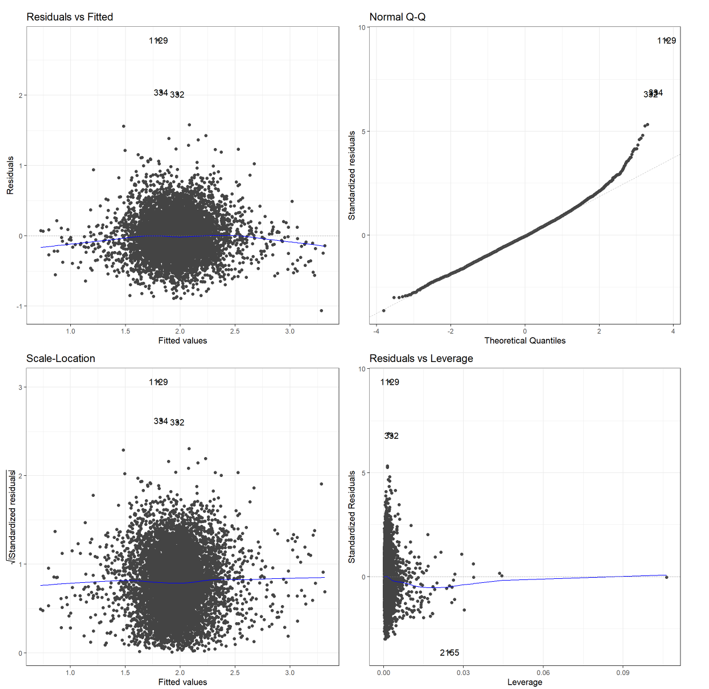
\includegraphics[width=0.95\linewidth]{figure/Figure_13} \caption{Diagnostics of OLS.}\label{fig:figure13}
\end{figure}
The OLS residual diagnostics above (Figure 5.12) do not appear to violate any OLS assumptions, although outliers are detected. Area 1129 is an area in Salford, while 334 and 332 surround Stamford Hill in inner London. The three areas host higher than expected TFR and appear to be practicing Jewish areas, a potential determinant that is excluded from the model. 2165 is a wealthy suburb of Bradford, West Yorkshire, and the reasoning for being an outlier in measuring leverage is unclear. The above diagnostics do not show any significant violation of OLS assumptions. The Farrar-Glauber test below provides overall multicollinearity diagnostics, and shows that collinearity is detected (Table 5.3).
\begin{table}

\caption{\label{tab:table4}Farrar-Glauber Test of Multicollinearity.}
\centering
\begin{tabu} to \linewidth {>{\raggedright}X>{\raggedleft}X>{\raggedleft}X}
\toprule
Test & MC Results & Detection\\
\midrule
Determinant |X'X| & 0.0427 & 0\\
Farrar Chi-Square & 22531.3604 & 1\\
Red Indicator & 0.2916 & 0\\
Sum of Lambda Inverse & 17.6465 & 0\\
Theil's Method & 0.7224 & 1\\
\addlinespace
Condition Number & 36.9762 & 1\\
\bottomrule
\multicolumn{3}{l}{\textsuperscript{} 0 - collinearity is not detected; 1 -}\\
\multicolumn{3}{l}{collinearity is detected.}\\
\end{tabu}
\end{table}
\begin{table}

\caption{\label{tab:table5}Individual collinearity.}
\centering
\begin{tabu} to \linewidth {>{\raggedright}X>{\raggedleft}X>{\raggedleft}X>{\raggedright}X>{\raggedleft}X}
\toprule
Variable & VIF & TOL & wi & Detection\\
\midrule
Education & 3.1028 & 0.3223 & 1890.1794 & 1\\
Pakistani & 1.3780 & 0.7257 & 339.8018 & 0\\
Bangladeshi & 1.2481 & 0.8012 & 222.9861 & 0\\
Black African & 1.7199 & 0.5814 & 647.1255 & 1\\
Income & 2.9781 & 0.3358 & 1778.0418 & 1\\
\addlinespace
Population Density (log) & 1.3767 & 0.7264 & 338.6303 & 0\\
Social Housing & 2.1327 & 0.4689 & 1018.1732 & 1\\
Divorce & 2.1591 & 0.4631 & 1941.9256 & 1\\
Non-Religiousness & 1.5510 & 0.6447 & 495.3020` & 0\\
\bottomrule
\multicolumn{5}{l}{\textsuperscript{} 0 - collinearity is not detected; 1 - collinearity is detected.}\\
\end{tabu}
\end{table}
Table 5.4 shows the output for the Variable Inflation Factor. The F-statistic for the university variable is highest (3.1028), followed by the income variable (2.9781), divorce (2.1591) and social housing (2.1327). This is an expected outcome and infers bias in oncoming results. Below, the normal distribution of residuals is shown (Figure 5.13). The right graph shows theoretical normal distribution in red, with the black line being the actual distribution. There is only a slight negative skew in the residuals. The residuals are also shown spatially in the following maps (Figure 5.14, 5.15), and the spatial clustering follows similar patterns as in the spatial dependence of TFR, suggesting that the causes of error and the causes of highly variant TFR are similar. Although the maps are informative and show clustering, the main result required is the Moran's I value of the residuals, 0.19 at a significance level of 0.001\%, thereby justifying the following spatial models.
\begin{figure}
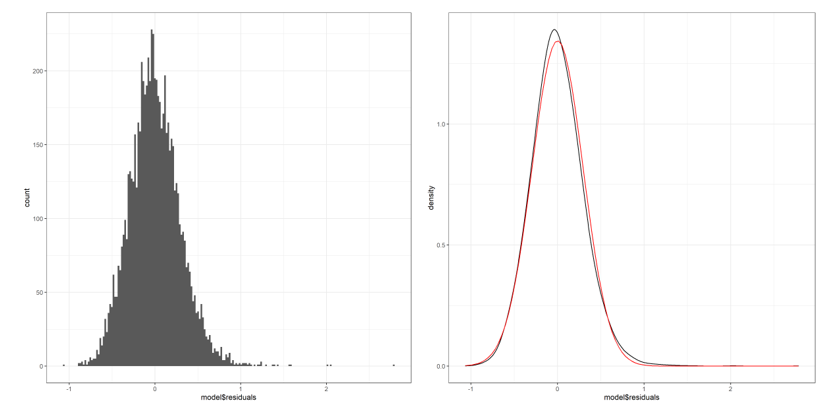
\includegraphics[width=0.95\linewidth]{figure/Figure_14} \caption{Normal Distribution in residuals.}\label{fig:figure14}
\end{figure}
\begin{figure}
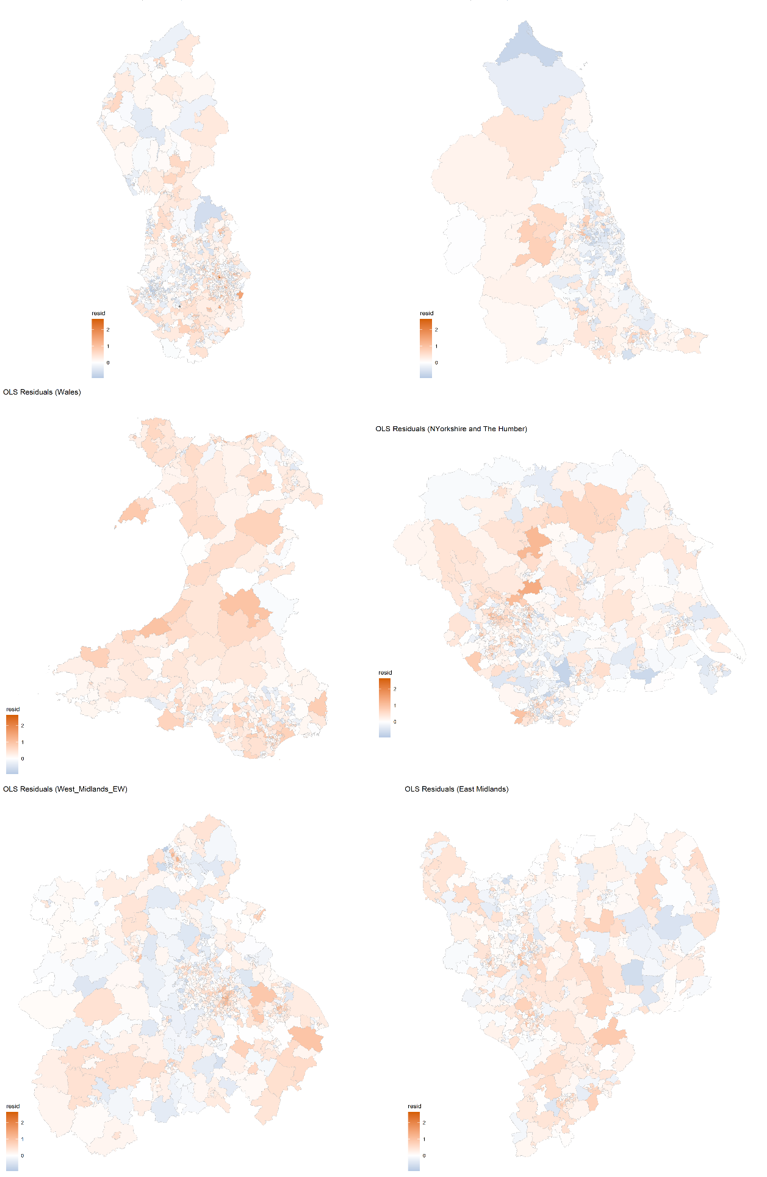
\includegraphics[width=0.95\linewidth]{figure/Figure_15} \caption{OLS Residuals. North West England (top left), North East England (top right), Wales (left), Yorkshire and the Humber (right), West Midlands (bottom left), East Midlands (bottom right). Boundary data source: UK data service, own depiction.}\label{fig:figure15}
\end{figure}
\begin{figure}
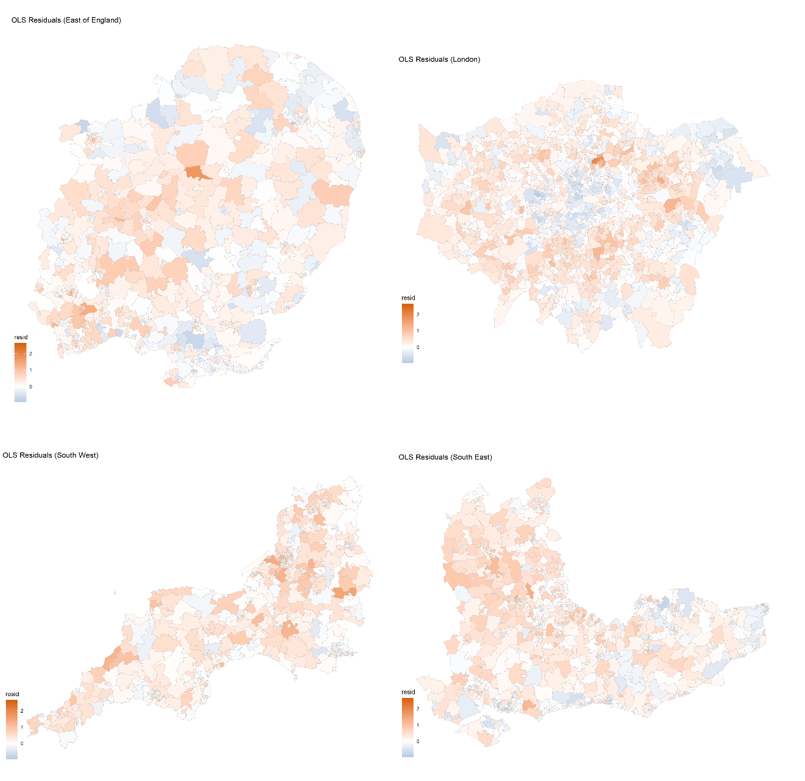
\includegraphics[width=0.95\linewidth]{figure/Figure_16} \caption{OLS Residuals. East of England (top left), London (top right), South West of England (bottom left), South East of England (bottom right). Boundary data source: UK data service, own depiction.}\label{fig:figure16}
\end{figure}
\hypertarget{addition-of-spatial-elements}{%
\section{Addition of Spatial Elements}\label{addition-of-spatial-elements}}

This section addresses the question: does the inclusion of a spatial autoregressive element to base OLS aid in the explanatory power of small-scale fertility outcomes, signifying the necessary inclusion of neighbour-to-neighbour fertility diffusion? In approaching the question, four models are built and briefly interpreted. As previously stated, the interpretation of spatial models with exogenous and endogenous effects differs from conventional least squares regression. The interpretation of the SAR model and SDM require differentiation between direct impacts, indirect impacts and total impacts, as the effects are no longer marginal and cannot be interpreted as such (LeSage, \protect\hyperlink{ref-lesage2008}{2008}; LeSage \& Pace, \protect\hyperlink{ref-lesage2006}{2006}). This is because the substantive effects of the explanatory variables are a result of different neighbourhood structures for each MSOA, that is, the effects of explanatory variables are different between MSOAs and therefore infer different neighbour-to-neighbour effects (Darmofal, \protect\hyperlink{ref-darmofal2015}{2015}). In essence, the direct impact is comparable to OLS interpretation, whereas the indirect impact is the influence of a neighbour's characteristics on an area's TFR. In contrast, the SEM contains no indirect effects as there is no spillover or loop, therefore, standard interpretation is possible (LeSage \& Pace, \protect\hyperlink{ref-lesage2018}{2018}).
\begin{table}

\caption{\label{tab:table6}Lag Model. Direct, Indirect and Total Effects (unstandardised).}
\centering
\fontsize{9}{11}\selectfont
\begin{tabu} to \linewidth {>{\centering}X>{\centering}X>{\centering}X>{\centering}X>{\centering}X>{\centering}X>{\centering}X}
\toprule
\multicolumn{1}{c}{ } & \multicolumn{2}{c}{Direct effects} & \multicolumn{2}{c}{Indirect effects} & \multicolumn{2}{c}{Total effects} \\
\cmidrule(l{3pt}r{3pt}){2-3} \cmidrule(l{3pt}r{3pt}){4-5} \cmidrule(l{3pt}r{3pt}){6-7}
  & $e^b$ & $e^b$*SE & $e^b$ & $e^b$*SE & $e^b$ & $e^b$*SE\\
\midrule
Education & -1.255*** & 0.04900 & -0.529*** & 0.03500 & -1.785*** & 0.0680\\
Pakistani & 1.798*** & 0.06800 & 0.759*** & 0.05000 & 2.557*** & 0.0960\\
Bangladeshi & 0.752*** & 0.01300 & 0.317*** & 0.05900 & 1.069*** & 0.1900\\
Black African & 1.484*** & 0.01900 & 0.626*** & 0.05700 & 2.11*** & 0.0650\\
Income & 0.001*** & 0.00005 & 0.0005*** & 0.00003 & 0.002*** & 0.0007\\
\addlinespace
Population Density (log) & -0.011*** & 0.00250 & -0.005*** & 0.00100 & -0.016*** & 0.0030\\
Social Housing & 0.302*** & 0.03800 & 0.127*** & 0.01900 & 0.428*** & 0.0560\\
Divorce & 6.136*** & 0.02900 & 2.589*** & 0.19300 & 8.726*** & 0.0380\\
Non-Religiousness & 0.028 & 0.03100 & 0.112 & 0.00300 & 0.039 & 0.0430\\
Intercept & 0.533*** & 0.04700 &  & NA &  & NA\\
\bottomrule
\multicolumn{7}{l}{\textsuperscript{} Rho (<U+03C1>): 0.3099. LR test value: 418.9***. AIC: 2549.}\\
\multicolumn{7}{l}{\textsuperscript{} *** P<0.001; ** p<0.01; * p <0.05.}\\
\multicolumn{7}{l}{\textsuperscript{} Source: ONS, own calculations.}\\
\end{tabu}
\end{table}
Neighbour-to-neighbour influence of fertility behaviours is shown in the SAR model by the significance of the \(\rho\) value (Table 5.5). This autoregressive parameter is highly significant, with the p-value \textless0.001 based on an asymptomatic t-test. The LR test value is 418.0, also with a highly significant p-value. The positive \(\rho\) value shows that when TFR increases in one area, as does the TFR in each neighbouring MSOA, and vice versa. When analysing the effects, the directional influence of each variable remains the same as in the OLS model, however, the magnitude is greater in each explanatory variable within the SAR model. As in the OLS model, only education and population density host negative influences on fertility, and non-religiousness remains non-significant. The direct and indirect impacts of population density are both negative, as is present regarding education. In all cases, the direct effect accounts for a greater proportion of the total effect than the indirect effects, and no variables show opposite impacts in direct and negative effects, being either both positive or both negative.
\begin{table}

\caption{\label{tab:table7}Error model compared to OLS model (unstandardised).}
\centering
\fontsize{9}{11}\selectfont
\begin{tabu} to \linewidth {>{\centering}X>{\centering}X>{\centering}X}
\toprule
  & SEM & OLS\\
\midrule
Intercept & 0.965*** & 1.097***\\
 & (-0.05) & (-0.041)\\
Education & -1.683*** & -1.6***\\
 & (-0.612) & (-0.049)\\
Pakistani & 2.112*** & 2.152***\\
\addlinespace
 & (-0.079) & (-0.069)\\
Bangladeshi & 1.089*** & 0.809***\\
 & (-0.166) & (-0.136)\\
Black African & 2.083*** & 2***\\
 & (-0.153) & (-0.122)\\
\addlinespace
Income & 0.00142*** & 0.001***\\
 & (-0.00006) & (-0.00003)\\
Population Density (log) & -0.00938*** & -0.012***\\
 & (-0.003) & (-0.0026)\\
Social Housing & 0.196*** & 0.193***\\
\addlinespace
 & (-0.043) & (-0.038)\\
Divorce & 6.671*** & 6.576***\\
 & (-0.283) & (-0.256)\\
Non-Religiousness & 0.197** & 0.018\\
 & (-0.075) & (-0.059)\\
\bottomrule
\multicolumn{3}{l}{\textsuperscript{} Lambda (<U+03BB>): 0.3877, LR test value: 555.9***. AIC:}\\
\multicolumn{3}{l}{2412.}\\
\multicolumn{3}{l}{\textsuperscript{} *** P<0.001; ** p<0.01; * p <0.05.}\\
\multicolumn{3}{l}{\textsuperscript{} Source: ONS, own calculations.}\\
\end{tabu}
\end{table}
The addition of the spatial autocorrelated error term (\(\lambda\)) is highly significant at the 0.001\% level at 0.387. The accompanying AIC is 2412, showing a large decrease and improvement in model fit from the previous SAR model. Generally, the strength of the coefficients are similar to the OLS model (Table 5.6, however, the contextual non-religious variable becomes significant and positive. Despite similarities between OLS and SEM, a spatial Hausman (Pace and LeSage, 2008) test shows that the regression parameter estimates themselves differ greatly (p\textless0.001) between the two models, in addition to increased model performance. In spite of seemingly useful results, this model does not directly relate to the research questions, as the model captures spatial clustering more so than social network effects. Similarly, the SDEM is far-removed from the research intention, but shows a similar model performance (Appendix 3).
\begin{table}

\caption{\label{tab:table8}Spatial Durbin Model. Direct, Indirect and Total Effects (unstandardised).}
\centering
\fontsize{9}{11}\selectfont
\begin{tabu} to \linewidth {>{\centering}X>{\centering}X>{\centering}X>{\centering}X>{\centering}X>{\centering}X>{\centering}X}
\toprule
\multicolumn{1}{c}{ } & \multicolumn{2}{c}{Direct effects} & \multicolumn{2}{c}{Indirect effects} & \multicolumn{2}{c}{Total effects} \\
\cmidrule(l{3pt}r{3pt}){2-3} \cmidrule(l{3pt}r{3pt}){4-5} \cmidrule(l{3pt}r{3pt}){6-7}
  & $e^b$ & $e^b$*SE & $e^b$ & $e^b$*SE & $e^b$ & $e^b$*SE\\
\midrule
Education & -1.757*** & 0.08500 & 0.276* & 0.1260 & -1.48*** & 0.09700\\
Pakistani & 2.072*** & 0.10300 & 0.234 & 0.1810 & 2.306*** & 0.14200\\
Bangladeshi & 1.639*** & 0.23800 & -1.248** & 0.3540 & 0.391 & 0.26900\\
Black African & 2.68*** & 0.24200 & -0.567 & 0.3390 & 2.112*** & 0.24300\\
Income & 0.002*** & 0.00009 & -0.0007*** & 0.0001 & 0.001*** & 0.00005\\
\addlinespace
Population Density (log) & -0.003 & 0.00300 & -0.017** & 0.0060 & -0.019*** & 0.00500\\
Social Housing & 0.223*** & 0.05200 & -0.039 & 0.0530 & 0.184 & 0.09800\\
Divorce & 6.564*** & 0.32900 & -0.099 & 0.7080 & 6.465*** & 0.64600\\
Non-Religiousness & 0.652*** & 0.09800 & -0.906*** & 0.1430 & -0.254* & 0.10700\\
Intercept & 0.801*** & 0.05700 &  & NA &  & NA\\
\bottomrule
\multicolumn{7}{l}{\textsuperscript{} Rho (<U+03C1>): 0.378. LR test value: 532.6***. AIC: 2325.}\\
\multicolumn{7}{l}{\textsuperscript{} *** P<0.001; ** p<0.01; * p <0.05.}\\
\multicolumn{7}{l}{\textsuperscript{} Source: ONS, own calculations.}\\
\end{tabu}
\end{table}
The interpretation of the SDM (as with the SAR model) is only different than OLS interpretation if \(\rho\) \(\not\equiv\) 0 (LeSage, \protect\hyperlink{ref-lesage2008}{2008}). The \(\rho\) value here is slightly higher than in the SAR model, at 0.378 and highly significant at the 0.001\% level. SDM models generally contain higher spillover (indirect effects) than other spatial models due to a wider inclusion of spatially lagged variables. The comparative SAR model indirect effects are similar but of lesser magnitude to the direct effects, whereas the direct and indirect effects in the SDM diverge.

In terms of interpreting the final chosen model, SDM, the direct impact of increased university-level education is significant and negatively associated with TFR. However, the indirect effect of increasing education in neighbouring regions is positive. This suggests that increased education in neighbouring MSOAs has a positive impact on TFR. This seems reasonable given education being positively associated with prosperous areas that may provide contextual incentives towards childbearing.

The direct effect of the Pakistani female population is significant and positive, suggesting an effect on TFR within a neighbourhood, \(i\). However, the indirect effect in neighbouring MSOAs is non-significant, suggesting an absence of neighbourhood effects relating to the Pakistani population, similarly seen in the Black African variable. In contrast, the direct effect of the Bangladeshi female population is positive and significant, suggesting that increased Bangladeshi proportions of neighbours leads to higher TFR. However, the indirect effects are negative, suggesting that areas neighbouring areas with large proportions of Bangladeshi women are influenced negatively in relation to TFR. The indirect impacts from the Bangladeshi population is roughly equal to that of the direct impact, resulting in a non-significant total impact due to these two effects balancing one another, an outcome also seen in the social housing variable.

Income appears to be one of the most significant variables both in direct and indirect effects. The direct effect of income leads to a positive and significant effect on TFR, however, the indirect effect of increased income in neighbouring MSOAs is negative and significant at the 0.01\% level. The total effect remains positive, but is lowered by the negative indirect effect. This opposes the compositional explanation for high educated areas influencing neighbours positively.

Population density hosts a non-significant effect in direct fertility, but the indirect effect on fertility is negative and positive. The social housing variable is dominated by the direct effects accounting for the vast majority of total effects. As proportion of social housing increases, as does the TFR of an area, however, the indirect influence of social housing on neighbours' TFR is non-significant. Divorce prevalence exerts a one-sided influence, with a positive direct effect on TFR suggesting an increase in fertility in areas with large divorced populations, yet the indirect effect is non-significant. Non-religious direct and indirect effects contradict one another as seen in the Bangladeshi variable. The direct effects of non-religiousness are significant and positive; however, the indirect effects are of a greater magnitude and negative. The resulting total effect is therefore negative, opposed to the OLS, SAR and SEM variables.
\begin{table}

\caption{\label{tab:table9}Model Comparison. Total Effects (unstandardised).}
\centering
\fontsize{9}{11}\selectfont
\begin{tabu} to \linewidth {>{\centering}X>{\centering}X>{\centering}X>{\centering}X>{\centering}X>{\centering}X}
\toprule
  & OLS & SAR & SEM & SDM & SDEM\\
\midrule
 &  &  &  &  & \\
Intercept & 1.097*** & 0.533*** & 0.965*** & -0.802*** & 1.185***\\
Education & -1.6*** & -1.78*** & -1.683*** & -1.484*** & -1.510***\\
Pakistani & 2.152*** & 2.557*** & 2.112*** & 2.306*** & 2.290***\\
Bangladeshi & 0.809*** & 1.068*** & 1.089*** & 0.391 & 0.581*\\
\addlinespace
Black African & 2*** & 2.110*** & 2.083*** & 2.112*** & 2.062***\\
Income & 0.001*** & 0.001*** & 0.001*** & 0.001*** & 0.002***\\
Population Density (log) & -0.012*** & -0.01*** & -0.009*** & -0.019*** & -0.017***\\
Social Housing & 0.193*** & 0.428*** & 0.196*** & 0.185 & 0.214*\\
Divorce & 6.576*** & 8.726*** & 6.671*** & 6.465*** & 7.028***\\
\addlinespace
Non-Religiousness & 0.018 & 0.039*** & 0.197** & -0.254* & -0.256*\\
 &  &  &  &  & \\
$\rho$ spatial parameter &  & 0.309 &  & 0.378 & \\
$\lambda$ spatial parameter &  &  & 0.387 &  & 0.381\\
AIC & 2966 & 2549 & 2412 & 2321 & 2325\\
\addlinespace
Adj. R2 & 0.401 &  &  &  & \\
\bottomrule
\multicolumn{6}{l}{\textsuperscript{a} *** P<0.001; ** p<0.01; * p <0.05}\\
\multicolumn{6}{l}{\textsuperscript{} standard errors available in earlier models; A Breusch-Pagan test reports heteroscedastity in all models at}\\
\multicolumn{6}{l}{p-values < 0.001.}\\
\multicolumn{6}{l}{\textsuperscript{} When using a more conservative studentized versions the issue remains: 130.4 for the SAR model, 29.3 for the}\\
\multicolumn{6}{l}{SEM, 88.6 for the SDM and 77.4 for the SDEM.}\\
\multicolumn{6}{l}{\textsuperscript{} Source: ONS, own calculations.}\\
\end{tabu}
\end{table}
In contrast to the SAR and SEM models, the variables Bangladeshi and social housing become non-significant when measuring total effects. Within different models and measuring separate impacts, the role of such variables is either positive or negative. In the SDM, both \(\rho\) and \(\lambda\) are significant, capturing both endogenous and exogenous spatial effects. The AIC of the SDM model is the lowest of all models, fitting well within the theoretical reasoning of this topic. The AIC fell from 2966 to 2549 with the addition of the spatially lagged TFR term. The theoretical background of this research requires the inclusion of a spatial autoregressive term in TFR, and the SDM captures this while also satisfying improvements in model performance.

\hypertarget{Discussion}{%
\chapter{Discussion}\label{Discussion}}

\hypertarget{limitations}{%
\section{Limitations}\label{limitations}}

The limitations of this dissertation largely refer to the data used and issues in modelling the drivers of spatial dependence. Compared to papers modelling fertility differentials within one socio-demographic classification (e.g.~cohabiting childbearing in Vitali et al., 2015), the analysis of TFR as a whole is difficult to draw conclusions from. TFR is a comparatively less accurate measure of fertility as compared to cohort fertility and tempo-adjusted rates (Kohler \& Ortega, \protect\hyperlink{ref-kohler2002a}{2002}). In addition, the birth and population data come from different sources, with the issue of migrant counts leading to potential over-estimations of TFR in areas of high short-term migration. The presence of students within an MSOA also distorts ASFRs and TFR due to MSOAs being small in size and students being geographically concentrated. There are also large fluctuations year-by-year in MSOA populations, and a possible small change in population would change ASFRs and TFR to a large degree.

Diffusion is temporal as well as spatial, and the use of panel data would allow time to be included, whereas the cross-sectional spatial econometric models included do not take time into account, assuming simultaneous changes throughout the model. The addition of time would allow for a more complex model to be built exploring the changes in spatial autocorrelation from 2002 to 2018, however, the number of available variables would decrease. Three spatial issues are clearly present. First, the identification of autocorrelation nay be mis-specified due to the arbitrary designation of polygons derived from census tracts (Anselin, \protect\hyperlink{ref-anselin1988}{1988}), referring to the Modifiable Areal Unit Problem caused by areal agglomeration (Fotheringham \& Wong, \protect\hyperlink{ref-fotheringham1991}{1991}). Under slightly different boundaries that more closely fit the notion of neighbourhood, the interpretation of the social processes would differ. That is, the spatial, diffusion-led methodology and results rely upon the 2011 MSOA boundaries being legitimate neighbourhoods. Second, the ecological fallacy is present, meaning aggregation leads to applying one variable value to multiple individuals. Third and similar to the Modifiable Areal Unit Problem, Galton's Problem refers to areas being similar to one another simply due to the boundaries drawn, rather than being independent observations and leading to a misspecification of interaction (Bivand et al., \protect\hyperlink{ref-bivand2013}{2013}).

\hypertarget{neighbour-to-neighbour-fertility-diffusion}{%
\section{Neighbour-to-neighbour fertility diffusion}\label{neighbour-to-neighbour-fertility-diffusion}}

The diffusion of fertility behaviours from neighbour-to-neighbour is significant within the models due to the impact of spatially lagged TFR improving model performance from the OLS to the SAR model, however, the significance is overshadowed in part by other spatial processes. In the aims and objectives section, it was hesitantly assumed that the spatial autocorrelation of TFR would have undergone significant changes between 2002 and 2018. Changes in the spatial dependence of ASFRs occurred, and the spatial autocorrelation of TFR increased, particularly following 2014. The significant spatial dependence of the OLS residuals answered question two in the Moran's I value of 0.19 and significance below the 0.001 level. The third research question became difficult to answer due to the borderline-significant RLMlag value, bringing into question whether spatial autoregression in TFR is as significant as anticipated and whether network effects are minimised due to boundaries drawn or a weakness of network effects. The primary results of the final, SDM model find education and ethnicity to be the key drivers in local fertility rates within England and Wales, and the compositional variables are more significant than the contextual variables, but the measurable strength of social networks cannot be intuitively derived. That is, population density and social housing are non-significant regarding the total effect of the model, although the total effect hides subtleties between the direct and indirect effects. The inclusion of lagged explanatory variables and associated indirect effects may be viewed as contextual influences in a neighbourhood affecting TFR elsewhere. The following discussion is largely split by the research questions; in descriptive, methodological and theoretical considerations.

The SDM provides a more nuanced view of local-scale drivers of fertility in separating direct form indirect effects. The difference between indirect and direct effects appears to be linked to the degree of compositional or contextual influence. That is, the neighbourhood (\(j\)) adjoined to an area (\(i\)) may influence the fertility intentions and behaviours of women and men in area \(i\). Therefore, the SDM direct and indirect effects may portray such outcomes, as indirect effects are not compositional and direct effects may be both. For instance, the role of education is negative within \(i\) as a largely compositional variable, however, when living next to an area (\(j\)) of increasing education level, the fertility outcomes of women in \(i\) increase. The fertility intentions and outcome differentials between immigrants and natives is well documented within England and Wales (Robards \& Berrington, \protect\hyperlink{ref-robards2016}{2016}), and the variance by ethnic group is shown in the highly significant direct effects within a neighbourhood but generally lacking indirect, contextual effects.

Fitting well-within recent changes in the relationship between GDP and fertility, income displays an overall positive effect on TFR. This differs from the bivariate analysis of TFR and income as well as the OLS model. When accounting for endogenous and exogenous spatial dependence, income is positively associated with TFR. As opposed to OLS, SAR and SEM results, the role of population density appears to be negative, in line with UK-based research (e.g., Kulu \& Washbrook, \protect\hyperlink{ref-kulu2014}{2014}). The role of indirect effects are highly significant, perhaps suggesting that the contextual effect of population density is highly linked to not only one neighbourhood, but also the surrounding areas. Divorce prevalence has a positive effect on fertility, potentially relating to a remarriage effect, however, the influence of a neighbour's divorce prevalence does not appear to be significant, deviating from network effect theory. Social housing also exerts only direct impact on TFR. The non-religious variable intends to show secularism and a loss of attachment to norms, and throughout the modelling process, non-religiousness is generally the weakest determinant, likely being useful in historic predictors of fertility but not applicable to contemporary contexts.

Spatial autocorrelation is not only derived from neighbours' influence, but also also arising from spatial dependence relating to a geographic and social clustering of similar behaviours (Darmofal, \protect\hyperlink{ref-darmofal2015}{2015}). The SEM captures this effect more so than any other model, and as seen in RLMlag test, the presence of neighbour-to-neighbour diffusion is less significant than network theory suggests. The RLMlag result alters the discourse, as diffusion cannot be confidently stated to be the driver of spatial dependence. Nonetheless, geography matters even without concretely identifying the exact spatial processes at the individual level. As famously stated by George Box, ``all models are wrong, but some are useful''. The models including error are not as useful or parsimonious as the SAR model or SDM which incorporate the spatial autoregression of fertility.

The context in which a social network is situated will affect the influence of fertility behaviours on others, and may determine the lesser significance when compared to other aggregate approaches in the literature. At the European regional scale, the spatial autoregression of TFR has been proven to be highly significant (Campisi et al., \protect\hyperlink{ref-campisi2020}{2020}). European wide research, and to an extent the scale of this dissertation, generalise social processes across the entire network. To clarify, Southern European networks are markedly close-knit and strong (Micheli, \protect\hyperlink{ref-micheli2000}{2000}) and therefore neighbour-to-neighbour transmission of fertility behaviours is expected to be more significant in Italy than in England and Wales. In the English and Welsh context, the determinants of fertility may be increasingly linked to individual, non-norm based effects, thereby causing social interactions to host less influence in a person's decision-making processes (Bernardi \& Klärner, \protect\hyperlink{ref-bernardi2014}{2014}). The 2011 model captures a snapshot of the two countries, where the diffusion of norms regarding non-marital childbirth and divorce is complete, with decisions now led largely by individual, rather than societal expectations. Therefore, the current diffusion process rests almost entirely on the social networks between individuals, households and neighbourhoods. However, these processes, and associated social contagion, do not appear to be as significant in the English and Welsh contexts as compared to less individual-led societies.

The central critique of European-wide approaches to fertility analysis is the whole-nation bias of aggregate macro-level comparison that oversimplifies and misdiagnoses demographic processes (Rokkan, \protect\hyperlink{ref-rokkan2009}{2009}). The sources of whole-nation bias are also present at the regional scale. The problem persists within this dissertation by analysing the 7,200 MSOAs of England and Wales simultaneously. Further research should aim to disaggregate the spatial processes by stratifications such as town, age group or ethnicity. Using similar methodologies in this dissertation but with parity-specific and age-specific data would be a natural next step. In overcoming whole-nation bias and trying to reduce the methodological distance to the individual processes, the research aims of the study could be analysed at the LSOA level - areas roughly one sixth the size of the current MSOA. The use of unaltered LSOA boundaries is impractical due to very low numbers of births and low populations. However, the combination of LSOAs based on shared characteristics could be an avenue for future research as done by Fiori et al. (\protect\hyperlink{ref-fiori2014}{2014}). Instead of agglomeration based on the rural/urban context as done by Fiori and colleagues, LSOAs could be combined to form more cohesive `neighbourhoods', which may overcome some error incurred from ONS aggregation methods

An alternative methodology to spatial econometrics that can identify the neighbourhood and social networks is agent-based modelling and simulation, which is becoming more common and mainstream in demographic research (Reinhardt, Hilton, Warnke, \& Bijak, \protect\hyperlink{ref-reinhardt2018}{2018}; Silverman, Bijak, Hilton, Cao, \& Noble, \protect\hyperlink{ref-silverman2013}{2013}). In future, a combination of methods is recommended, namely with the addition of agent-based modelling in taking the macro-level approach to the meso- and micro-level, where the processes of social contagion take place and the idea of a neighbourhood formulated. The role of space and spatial dependence is highly significant in fertility outcomes, and in moving closer to the individual, this research has bridged a gap between the micro- and macro-scale. The main question that needs to be addressed further relates to why social network influence is not as stark as theories suggest, and whether intricacies exist within groups of the population. Socio-demographic compositional variables are the dominant determinants of fertility outcomes, while contextual variables are comparatively weak. Despite being central, individual characteristics do not explain fertility outcomes alone, taking place alongside increasingly complicated spatial processes.

\appendix

\hypertarget{appendix}{%
\chapter*{Appendix}\label{appendix}}
\addcontentsline{toc}{chapter}{Appendix}
\begin{table}

\caption{\label{tab:appendix1}Appendix 1. Bivariate correlation and p-values.}
\centering
\fontsize{9}{11}\selectfont
\begin{tabu} to \linewidth {>{\centering}X>{\centering}X>{\centering}X>{\centering}X>{\centering}X>{\centering}X>{\centering}X>{\centering}X>{\centering}X>{\centering}X}
\toprule
Variable & TFR & EDU & Pakistani & Bangladeshi & Black.African & INC & LOGPDENS & SOCHO & DIV\\
\midrule
TFR &  &  &  &  &  &  &  &  & \\
EDU & -0.447*** &  &  &  &  &  &  &  & \\
Pakistani & 0.297*** & -0.099*** &  &  &  &  &  &  & \\
Bangladeshi & 0.109*** & 0.011 & 0.281*** &  &  &  &  &  & \\
Black African & 0.195*** & 0.06*** & 0.14*** & 0.236*** &  &  &  &  & \\
\addlinespace
INC & -0.259*** & 0.779*** & -0.128*** & -0.042*** & 0.02 &  &  &  & \\
LOGPDENS & 0.117*** & -0.028* & 0.229*** & 0.238*** & 0.403*** & -0.086*** &  &  & \\
SOCHO & 0.302*** & -0.373*** & 0.068*** & 0.211*** & 0.476*** & -0.461*** & 0.373*** &  & \\
DIV & 0.323*** & -0.563*** & -0.247*** & -0.213*** & -0.151*** & -0.528*** & -0.037** & 0.329*** & \\
NONRG & -0.092*** & 0.04*** & -0.365*** & -0.24*** & -0.176*** & -0.084*** & 0.055*** & 0.123*** & 0.371***\\
\bottomrule
\multicolumn{10}{l}{\textsuperscript{} *** P<0.001; ** p<0.01; * p <0.05}\\
\multicolumn{10}{l}{\textsuperscript{} Source: ONS, own calculations.}\\
\end{tabu}
\end{table}
\begin{figure}
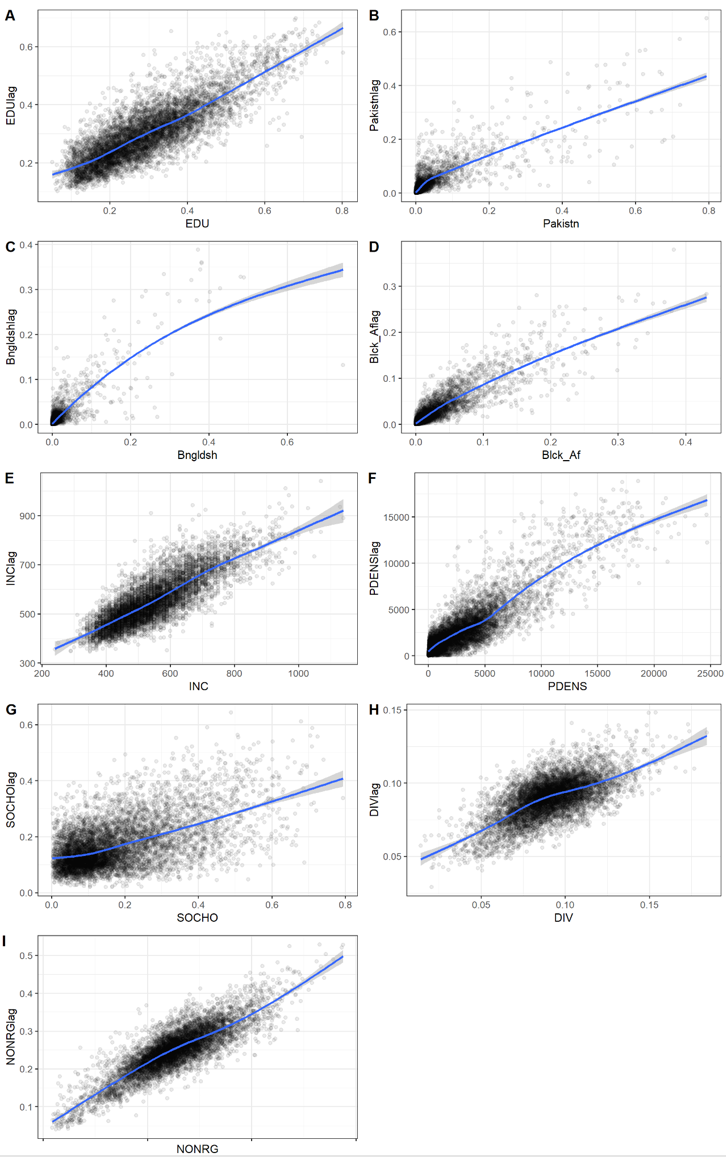
\includegraphics[width=0.95\linewidth]{figure/Appendix_2} \caption{Appendix 2. Spatial autocorrelation of explanatory variables. Source: ONS, own calculations.}\label{fig:appendix2}
\end{figure}
\begin{table}

\caption{\label{tab:appendix3}Appendix 3. Spatial Durbin Error Model. Direct, Indirect and Total Effects (unstandardised.}
\centering
\fontsize{9}{11}\selectfont
\begin{tabu} to \linewidth {>{\centering}X>{\centering}X>{\centering}X>{\centering}X>{\centering}X>{\centering}X>{\centering}X}
\toprule
\multicolumn{1}{c}{ } & \multicolumn{2}{c}{Direct effects} & \multicolumn{2}{c}{Indirect effects} & \multicolumn{2}{c}{Total effects} \\
\cmidrule(l{3pt}r{3pt}){2-3} \cmidrule(l{3pt}r{3pt}){4-5} \cmidrule(l{3pt}r{3pt}){6-7}
  & $e^b$ & $e^b$*SE & $e^b$ & $e^b$*SE & $e^b$ & $e^b$*SE\\
\midrule
Education & -1.709*** & 0.08100 & 0.198 & 0.1160 & -1.510 & -1.51***\\
Pakistani & 2.055*** & 0.10100 & 0.235 & 0.1640 & 2.290 & 2.29***\\
Bangladeshi & 1.564*** & 0.21100 & -0.982* & 0.3150 & 0.581 & 0.581*\\
Black African & 2.629*** & 0.21600 & -0.564 & 0.2950 & 2.065 & 2.065***\\
Income & 0.002*** & 0.00008 & -0.0006*** & 0.0001 & 0.001 & 0.001***\\
\addlinespace
Population Density (log) & -0.003 & 0.00400 & -0.014* & 0.0060 & -0.017 & -0.017***\\
Social Housing & 0.229*** & 0.04900 & -0.015 & 0.0850 & 0.214 & 0.214*\\
Divorce & 6.46*** & 0.31000 & 0.567 & 0.5510 & 7.027 & 7.027***\\
Non-Religiousness & 0.667*** & 0.10300 & -0.923*** & 0.1370 & -0.251 & -0.251*\\
Intercept & 1.185*** & 0.07800 &  & NA & NA & \\
\bottomrule
\multicolumn{7}{l}{\textsuperscript{} Lambda: 0.381 (<U+03BB>). LR test value: 538.9***. AIC: 2330.8.}\\
\multicolumn{7}{l}{\textsuperscript{} *** P<0.001; ** p<0.01; * p <0.05.}\\
\multicolumn{7}{l}{\textsuperscript{} Source: ONS, own calculations.}\\
\end{tabu}
\end{table}
\backmatter

\hypertarget{references}{%
\chapter*{References}\label{references}}
\addcontentsline{toc}{chapter}{References}

\markboth{References}{References}

\noindent

\setlength{\parindent}{-0.20in}
\setlength{\leftskip}{0.20in}
\setlength{\parskip}{8pt}

Bivand, R. 2019. Analysis of Spatial Data. {[}Online{]}. \url{https://cran.r-project.org/web/views/Spatial.html}.

ONS. 2018. Live births by age of mother, 2000 to 2016: England and Wales. Online. Available from: \url{https://www.ons.gov.uk/peoplepopulationandcommunity/birthsdeathsandmarriages/livebirths/adhocs/008072livebirthsbyageofmotherandfather2000to2016englandandwales}.

ONS, 2019a. Birth characteristics in England and Wales: 2017. {[}Online{]}. \url{https://www.ons.gov.uk/peoplepopulationandcommunity/birthsdeathsandmarriages/livebirths/bulletins/birthcharacteristicsinenglandandwales/2017}.

ONS, 2019b. Births by Lower layer Super Output Area (LSOA), England and Wales, mid-year 2001 to 2018. {[}Online{]}. \url{https://www.ons.gov.uk/peoplepopulationandcommunity/birthsdeathsandmarriages/livebirths/adhocs/10773birthsbylowerlayersuperoutputarealsoaenglandandwalesmidyear2001to2018}.

ONS, 2020a. Income estimates for small areas, England and Wales. {[}Online{]}. \url{https://www.ons.gov.uk/employmentandlabourmarket/peopleinwork/earningsandworkinghours/datasets/smallareaincomeestimatesformiddlelayersuperoutputareasenglandandwales}

ONS, 2020b. Lower layer Super Output Area Population estimates. {[}Online{]}. \url{https://www.ons.gov.uk/peoplepopulationandcommunity/populationandmigration/populationestimates/datasets/lowersuperoutputareamidyearpopulationestimates}.

ONS. 2016. Census geography: An overview of the various geographies used in the production of statistics collected via the UK census. {[}Online{]}. \url{https://www.ons.gov.uk/methodology/geography/ukgeographies/censusgeography}

ONS. 2018. Live births by age of mother, 2000 to 2016: England and Wales. {[}Online{]}. Available from: \url{https://www.ons.gov.uk/peoplepopulationandcommunity/birthsdeathsandmarriages/livebirths/adhocs/008072livebirthsbyageofmotherandfather2000to2016englandandwales}.

Fiori, F. 2020. Social disparities in residential mobility and children's outcomes in early and middle childhood. Presentation at the British Population Society for Population Studies, 2020.

Jaadla, Ried, Garrett. 2020. Continuity and change in spatial patterns in UK fertility: the case of London. Presentation at the British Population Society for Population Studies BSPS Conference, 2020. Online.

\hypertarget{refs}{}
\leavevmode\hypertarget{ref-akaike1974}{}%
Akaike, H. (1974). A new look at the statistical model identification. \emph{IEEE Transactions on Automatic Control}, \emph{19}(6), 716--723.

\leavevmode\hypertarget{ref-anselin1988}{}%
Anselin, L. (1988). Spatial Econometrics: Methods and Models.

\leavevmode\hypertarget{ref-anselin1995}{}%
Anselin, L. (1995). Local indicators of spatial associationLISA. \emph{Geographical Analysis}, \emph{27}(2), 93--115.

\leavevmode\hypertarget{ref-anselin1996}{}%
Anselin, L., Bera, A. K., Florax, R., \& Yoon, M. J. (1996). Simple diagnostic tests for spatial dependence. \emph{Regional Science and Urban Economics}, \emph{26}(1), 77--104.

\leavevmode\hypertarget{ref-balbo2014}{}%
Balbo, N., \& Barban, N. (2014). Does Fertility Behavior Spread among Friends? \emph{American Sociological Review}, \emph{79}(3), 412--431. \url{http://doi.org/10.1177/0003122414531596}

\leavevmode\hypertarget{ref-basten2011}{}%
Basten, S., Huinink, J., \& Klüsener, S. (2011). Spatial variation of sub-national fertility trends in Austria, Germany and Switzerland. \emph{Comparative Population Studies}, \emph{36}(2-3), 573--614. \url{http://doi.org/10.4232/10.CPoS-2011-08en}

\leavevmode\hypertarget{ref-bavaud1998}{}%
Bavaud, F. (1998). Models for spatial weights: A systematic look. \emph{Geographical Analysis}, \emph{30}(2), 153--171.

\leavevmode\hypertarget{ref-becker1981}{}%
Becker, G. (1981). A Treatise on the Family.

\leavevmode\hypertarget{ref-bera1993}{}%
Bera, A. K., \& Yoon, M. J. (1993). Specification testing with locally misspecified alternatives. \emph{Econometric Theory}, 649--658.

\leavevmode\hypertarget{ref-bernardi2007}{}%
Bernardi, L., Keim, S., \& Von Der Lippe, H. (2007). Social Influences on Fertility: A Comparative Mixed Methods Study in Eastern and Western Germany. \emph{Journal of Mixed Methods Research}, \emph{1}(1), 23--47. \url{http://doi.org/10.1177/2345678906292238}

\leavevmode\hypertarget{ref-bernardi2014}{}%
Bernardi, L., \& Klärner, A. (2014). Social networks and fertility. \emph{Demographic Research}, \emph{30}, 641--670.

\leavevmode\hypertarget{ref-bernhardt2004}{}%
Bernhardt, E. (2004). Is the Second Demographic Transition a useful concept for demography? \emph{Vienna Yearbook of Population Research}, \emph{2}, 25--28.

\leavevmode\hypertarget{ref-berrington2014}{}%
Berrington, A., \& Pattaro, S. (2014). Educational differences in fertility desires, intentions and behaviour: A life course perspective. \emph{Advances in Life Course Research}, \emph{21}, 10--27.

\leavevmode\hypertarget{ref-billari2012}{}%
Billari, F. C., \& Dalla-Zuanna, G. (2012). Is replacement migration actually taking place in low fertility countries? \emph{Genus}, \emph{67}(3).

\leavevmode\hypertarget{ref-bivand2013}{}%
Bivand, R., Pebesma, E., \& Gómez-Rubio, V. (2013). Applied Spatial Data Analysis with R.

\leavevmode\hypertarget{ref-blossfeld1991}{}%
Blossfeld, H.-P., \& Huinink, J. (1991). Human capital investments or norms of role transition? How women's schooling and career affect the process of family formation. \emph{American Journal of Sociology}, \emph{97}(1), 143--168.

\leavevmode\hypertarget{ref-bongaarts1996}{}%
Bongaarts, J., \& Watkins, S. C. (1996). Social interactions and contemporary fertility transitions. \emph{Population and Development Review}, 639--682.

\leavevmode\hypertarget{ref-boyle2007}{}%
Boyle, P. J., Graham, E., \& Feng, Z. (2007). Contextualising Demography : The Significance of Local Clusters of Fertility in Scotland, \emph{49}(0), 0--39. \url{http://doi.org/10.4054/MPIDR-WP-2007-036}

\leavevmode\hypertarget{ref-bryan2016}{}%
Bryan, M. L., \& Jenkins, S. P. (2016). Multilevel modelling of country effects: A cautionary tale. \emph{European Sociological Review}, \emph{32}(1), 3--22. \url{http://doi.org/10.1093/esr/jcv059}

\leavevmode\hypertarget{ref-buber2000}{}%
Buber, I., \& Prskawetz, A. (2000). Fertility in second unions in Austria: Findings from the Austrian FFS. \emph{Demographic Research}, \emph{3}.

\leavevmode\hypertarget{ref-bujard2017}{}%
Bujard, M., \& Scheller, M. (2017). Impact of Regional Factors on Cohort Fertility: New Estimations at the District Level in Germany. \emph{Comparativepopulationstudies.de}, \emph{42}, 55--88. \url{http://doi.org/10.12765/CPoS-2017-08en}

\leavevmode\hypertarget{ref-campisi2020}{}%
Campisi, N., Kulu, H., Mikolai, J., Klüsener, S., \& Myrskylä, M. (2020). Spatial variation in fertility across Europe: Patterns and determinants. \emph{Population, Space and Place}, \emph{26}(4). \url{http://doi.org/10.1002/psp.2308}

\leavevmode\hypertarget{ref-casterline2001}{}%
Casterline, J. B., \& Washington, D. C. (2001). \emph{SELECTED PERSPECTIVES Committee on Population DIFFUSION PROCESSES FERTILITY TRANSITION}.

\leavevmode\hypertarget{ref-corrado2012}{}%
Corrado, L., \& Fingleton, B. (2012). Where is the economics in spatial econometrics? \emph{Journal of Regional Science}, \emph{52}(2), 210--239. \url{http://doi.org/10.1111/j.1467-9787.2011.00726.x}

\leavevmode\hypertarget{ref-darmofal2015}{}%
Darmofal, D. (2015). \emph{Spatial analysis for the social sciences}. Cambridge University Press.

\leavevmode\hypertarget{ref-debeer2007}{}%
de Beer, J., \& Deerenberg, I. (2007). An explanatory model for projecting regional fertility differences in the Netherlands. \emph{Population Research and Policy Review}, \emph{26}(5-6), 511--528. \url{http://doi.org/10.1007/s11113-007-9040-y}

\leavevmode\hypertarget{ref-diaz2011}{}%
Diaz, B. A., Fent, T., Prskawetz, A., \& Bernardi, L. (2011). Transition to Parenthood: The Role of Social Interaction and Endogenous Networks. \emph{Demography}, \emph{48}(2), 559--579. \url{http://doi.org/10.1007/s13524-011-0023-6}

\leavevmode\hypertarget{ref-dormann2007}{}%
Dormann, C. F., M. McPherson, J., B. Araújo, M., Bivand, R., Bolliger, J., Carl, G., \ldots{} Daniel Kissling, W. (2007). Methods to account for spatial autocorrelation in the analysis of species distributional data: A review. \emph{Ecography}, \emph{30}(5), 609--628.

\leavevmode\hypertarget{ref-dubuc2009}{}%
Dubuc, S. (2009). Application of the Own-Children Method for estimating fertility by ethnic and religious groups in the UK. \emph{Journal of Population Research}, \emph{26}(3), 207--225.

\leavevmode\hypertarget{ref-dubuc2012}{}%
Dubuc, S. (2012). Immigration to the UK from high-fertility countries: Intergenerational adaptation and fertility convergence. \emph{Population and Development Review}, \emph{38}(2), 353--368.

\leavevmode\hypertarget{ref-durlauf2001}{}%
Durlauf, S. N., \& Walker, J. (2001). Social interactions and fertility transitions. \emph{Diffusion Processes and Fertility Transition: Selected Perspectives}, 115--137.

\leavevmode\hypertarget{ref-ekert-jaffe2002}{}%
Ekert-Jaffé, O., Joshi, H., Lynch, K., Mougin, R., \& Rendall, M. (2002). Fertility, timing of births and socio-economic status in France and Britain: Social policies and occupational polarization. \emph{Population}, \emph{57}(3), 475--508. \url{http://doi.org/10.2307/3246636}

\leavevmode\hypertarget{ref-elhorst2014}{}%
Elhorst, J. P. (2014). \emph{Spatial econometrics: From cross-sectional data to spatial panels} (Vol. 479). Springer.

\leavevmode\hypertarget{ref-fent2013}{}%
Fent, T., Diaz, B. A., \& Prskawetz, A. (2013). Family policies in the context of low fertility and social structure. \emph{Demographic Research}, \emph{29}, 963--998.

\leavevmode\hypertarget{ref-fiori2014}{}%
Fiori, F., Graham, E., \& Feng, Z. (2014). Geographical variations in fertility and transition to second and third birth in Britain. \emph{Advances in Life Course Research}, \emph{21}, 149--167.

\leavevmode\hypertarget{ref-fotheringham1991}{}%
Fotheringham, A. S., \& Wong, D. W. (1991). The modifiable areal unit problem in multivariate statistical analysis. \emph{Environment and Planning A}, \emph{23}(7), 1025--1044.

\leavevmode\hypertarget{ref-fox2019}{}%
Fox, J., Klüsener, S., \& Myrskylä, M. (2019). Is a Positive Relationship Between Fertility and Economic Development Emerging at the Sub-National Regional Level? Theoretical Considerations and Evidence from Europe. \emph{European Journal of Population}, \emph{35}(3), 487--518. \url{http://doi.org/10.1007/s10680-018-9485-1}

\leavevmode\hypertarget{ref-goldstein2013}{}%
Goldstein, J., Karaman Örsal, D. D., Kreyenfeld, M., \& Jasilioniene, A. (2013). Fertility Reactions to the "Great Recession" in Europe: Recent Evidence from Order-Specific Data. \emph{Demographic Research}, \emph{29}, 85--104. \url{http://doi.org/10.4054/DemRes.2013.29.4}

\leavevmode\hypertarget{ref-goldstein2014}{}%
Goldstein, J. R., \& Klüsener, S. (2014). Spatial analysis of the causes of fertility decline in Prussia. \emph{Population and Development Review}, \emph{40}(3), 497--525. \url{http://doi.org/10.1111/j.1728-4457.2014.00695.x}

\leavevmode\hypertarget{ref-golgher2016}{}%
Golgher, A. B., \& Voss, P. R. (2016). How to interpret the coefficients of spatial models: Spillovers, direct and indirect effects. \emph{Spatial Demography}, \emph{4}(3), 175--205.

\leavevmode\hypertarget{ref-granovetter1973}{}%
Granovetter, M. S. (1973). The strength of weak ties. \emph{American Journal of Sociology}, \emph{78}(6), 1360--1380.

\leavevmode\hypertarget{ref-gray2018}{}%
Gray, E., \& Evans, A. (2018). Geographic variation in parity progression in Australia. \emph{Population, Space and Place}, \emph{24}(2). \url{http://doi.org/10.1002/psp.2080}

\leavevmode\hypertarget{ref-hank2001}{}%
Hank, K. (2001). Regional fertility differences in Western Germany: An overview of the literature and recent descriptive findings. \emph{International Journal of Population Geography}, \emph{7}(4), 243--257. \url{http://doi.org/10.1002/ijpg.228}

\leavevmode\hypertarget{ref-haque2019}{}%
Haque, I., Das, D., \& Patel, P. (2019). Reading the geography of India's district-level fertility differentials: A spatial econometric approach. \emph{Journal of Biosocial Science}.

\leavevmode\hypertarget{ref-harris2009}{}%
Harris, R. (2009). \emph{In Search of 'W'}. \emph{rsa.tandfonline.com}.

\leavevmode\hypertarget{ref-jaadla2018}{}%
Jaadla, H., Reid, A., \& Garrett, E. (2018). \emph{Mobility, social class and fertility transition in England and Wales, 1851-1911 1}. \emph{Annual Meeting of the Population Association of America, Denver, CO}.

\leavevmode\hypertarget{ref-jalovaara2019}{}%
Jalovaara, M., Neyer, G., Andersson, G., Dahlberg, J., Dommermuth, L., Fallesen, P., \& Lappeg\textbackslash aard, T. (2019). Education, gender, and cohort fertility in the Nordic countries. \emph{European Journal of Population}, \emph{35}(3), 563--586.

\leavevmode\hypertarget{ref-jefferies2000}{}%
Jefferies, J., Berrington, A., \& Diamond, I. (2000). Childbearing following marital dissolution in Britain. \emph{European Journal of Population/Revue Européenne de Démographie}, \emph{16}(3), 193--210.

\leavevmode\hypertarget{ref-jemna2018}{}%
Jemna, D.-V., \& David, M. (2018). Post-transitional regional fertility in Romania. \emph{DEMOGRAPHIC RESEARCH}, \emph{38}. \url{http://doi.org/10.4054/DemRes.2018.38.57}

\leavevmode\hypertarget{ref-jeronimomuniz2006}{}%
Jeronimo Muniz. (2006). Spatial dependence and heterogeneity in ten years of fertility decline in Brazil : Where , why and how fast. \emph{Population Association of America 2006 Annual Meeting}, \emph{48}(2), 1--46.

\leavevmode\hypertarget{ref-jung2019}{}%
Jung, M., Ko, W., Choi, Y., \& Cho, Y. (2019). Spatial variations in fertility of South Korea: A geographically weighted regression approach. \emph{ISPRS International Journal of Geo-Information}, \emph{8}(6), 262--262. \url{http://doi.org/10.3390/ijgi8060262}

\leavevmode\hypertarget{ref-klusener2019}{}%
Klüsener, S., Dribe, M., \& Scalone, F. (2019). Spatial and Social Distance at the Onset of the Fertility Transition: Sweden, 18801900. \emph{Demography}, \emph{56}(1), 169--199. \url{http://doi.org/10.1007/s13524-018-0737-9}

\leavevmode\hypertarget{ref-klusener2013}{}%
Klüsener, S., Neels, K., \& Kreyenfeld, M. (2013). \emph{Family Policies and the Western European Fertility Divide: Insights from a Natural Experiment in Belgium} (No. 4). \emph{Source: Population and Development Review} (Vol. 39, pp. 587--610).

\leavevmode\hypertarget{ref-kohler2002b}{}%
Kohler, H., Billari, F., development, J. O. P. and, \& 2002, undefined. (2002). The emergence of lowest-low fertility in Europe during the 1990s. \emph{Population and Development Review}, \emph{28}(4), 641--680.

\leavevmode\hypertarget{ref-kohler2002a}{}%
Kohler, H.-P., \& Ortega, J. A. (2002). Tempo-adjusted period parity progression measures, fertility postponement and completed cohort fertility. \emph{Demographic Research}, \emph{6}, 91--144.

\leavevmode\hypertarget{ref-kondo2016}{}%
Kondo, K. (2016). \emph{Introduction to spatial econometric analysis: Creating spatially lagged variables in Stata}. RIETI.

\leavevmode\hypertarget{ref-kulu2013}{}%
Kulu, H. (2013). Why Do Fertility Levels Vary between Urban and Rural Areas? \emph{Regional Studies}, \emph{47}(6), 895--912. \url{http://doi.org/10.1080/00343404.2011.581276}

\leavevmode\hypertarget{ref-kulu2009}{}%
Kulu, H., \& Boyle, P. J. (2009). High fertility in city suburbs: Compositional or contextual effects? \emph{European Journal of Population/Revue Européenne de Démographie}, \emph{25}(2), 157--174.

\leavevmode\hypertarget{ref-kulu2007}{}%
Kulu, H., \& Vikat, A. (2007). Fertility differences by housing type. \emph{Demographic Research}, \emph{17}, 775--802. \url{http://doi.org/10.4054/demres.2007.17.26}

\leavevmode\hypertarget{ref-kulu2014}{}%
Kulu, H., \& Washbrook, E. (2014). Residential context, migration and fertility in a modern urban society. \emph{Advances in Life Course Research}, \emph{21}, 168--182. \url{http://doi.org/10.1016/j.alcr.2014.01.001}

\leavevmode\hypertarget{ref-lesage2008}{}%
LeSage, J. P. (2008). An Introduction to Spatial Econometrics. \emph{Revue d'économie Industrielle}, (123), 19--44. \url{http://doi.org/10.4000/rei.3887}

\leavevmode\hypertarget{ref-lesage2014a}{}%
LeSage, J. P. (2014). What regional scientists need to know about spatial econometrics. \emph{Available at SSRN 2420725}.

\leavevmode\hypertarget{ref-lesage2006}{}%
LeSage, J. P., \& Pace, R. K. (2006). Interpreting Spatial Econometric Models 77. \emph{Handbook of Regional Science}, 1535.

\leavevmode\hypertarget{ref-lesage2010}{}%
LeSage, J. P., \& Pace, R. K. (2010). Spatial econometric models. In \emph{Handbook of applied spatial analysis} (pp. 355--376). Springer.

\leavevmode\hypertarget{ref-lesage2014}{}%
LeSage, J. P., \& Pace, R. K. (2014). The biggest myth in spatial econometrics. \emph{Econometrics}, \emph{2}(4), 217--249.

\leavevmode\hypertarget{ref-lesage2018}{}%
LeSage, J. P., \& Pace, R. K. (2018). Spatial econometric Monte Carlo studies: Raising the bar. \emph{Empirical Economics}, \emph{55}(1), 17--34.

\leavevmode\hypertarget{ref-lesthaeghe1995}{}%
Lesthaeghe, R. (1995). The Second Demographic Transition in Western Countries: An Interpretation. \emph{Gender and Family Change in Industrialized Countries}, (August), 17--62. \url{http://doi.org/10.2307/1534906}

\leavevmode\hypertarget{ref-lois2014}{}%
Lois, D., \& Arránz Becker, O. (2014). Is fertility contagious? Using panel data to disentangle mechanisms of social network influences on fertility decisions. \emph{Advances in Life Course Research}, \emph{21}, 123--134. \url{http://doi.org/10.1016/j.alcr.2013.10.001}

\leavevmode\hypertarget{ref-lutz2011}{}%
Lutz, W., \& Samir, K. C. (2011). Global human capital: Integrating education and population. \emph{Science}, \emph{333}(6042), 587--592.

\leavevmode\hypertarget{ref-manski1993}{}%
Manski, C. F. (1993). Dynamic choice in social settings: Learning from the experiences of others. \emph{Journal of Econometrics}, \emph{58}(1-2), 121--136.

\leavevmode\hypertarget{ref-micheli2000}{}%
Micheli, G. A. (2000). Kinship, family and social network: The anthropological embedment of fertility change in Southern Europe. \emph{Demographic Research}, \emph{3}.

\leavevmode\hypertarget{ref-myrskyla2011a}{}%
Myrskylä, M., Kohler, H.-P., \& Billari, F. (2011). High development and fertility: Fertility at older reproductive ages and gender equality explain the positive link.

\leavevmode\hypertarget{ref-nisen2020}{}%
Nisén, J., Klüsener, S., Dahlberg, J., Dommermuth, L., Jasilioniene, A., Kreyenfeld, M., \ldots{} Myrskylä, M. (2020). Educational Differences in Cohort Fertility Across Sub-national Regions in Europe. \emph{European Journal of Population}, 1--33. \url{http://doi.org/10.1007/s10680-020-09562-0}

\leavevmode\hypertarget{ref-nibhrolchain2012}{}%
Ní Bhrolcháin, M., \& Beaujouan, É. (2012). Fertility postponement is largely due to rising educational enrolment. \emph{Population Studies}, \emph{66}(3), 311--327. \url{http://doi.org/10.1080/00324728.2012.697569}

\leavevmode\hypertarget{ref-prskawetz2003}{}%
Prskawetz, A., Vikat, A., Philipov, D., \& Engelhardt, H. (2003). Pathways to stepfamily formation in Europe: Results from the FFS. \emph{Demographic Research}, \emph{8}, 107--150.

\leavevmode\hypertarget{ref-reinhardt2018}{}%
Reinhardt, O., Hilton, J., Warnke, T., \& Bijak, J. (2018). Streamlining simulation experiments with agent-based models in demography. \emph{Jasss.soc.surrey.ac.uk}.

\leavevmode\hypertarget{ref-rendall2009}{}%
Rendall, M. S., Ekert-Jaffé, O., Joshi, H., Lynch, K., \& Mougin, R. (2009). Universal versus economically polarized change in age at first birth: A French - British comparison. \emph{Population and Development Review}, \emph{35}(1), 89--115. \url{http://doi.org/10.1111/j.1728-4457.2009.00262.x}

\leavevmode\hypertarget{ref-robards2016}{}%
Robards, J., \& Berrington, A. (2016). The fertility of recent migrants to England and Wales. \emph{Demographic Research}, \emph{34}, 1037--1052.

\leavevmode\hypertarget{ref-rokkan2009}{}%
Rokkan, S. (2009). \emph{Citizens, elections, parties: Approaches to the comparative study of the processes of development}. ECPR Press.

\leavevmode\hypertarget{ref-rossier2009}{}%
Rossier, C., \& Bernardi, L. (2009). Social interaction effects on fertility: Intentions and behaviors. \emph{European Journal of Population/Revue Européenne de Démographie}, \emph{25}(4), 467--485.

\leavevmode\hypertarget{ref-schoen1999b}{}%
Schoen, R., Astone, N. M., Kim, Y. J., Nathanson, C. A., \& Fields, J. M. (1999). Do fertility intentions affect fertility behavior? \emph{Journal of Marriage and the Family}, 790--799.

\leavevmode\hypertarget{ref-sigle-rushton2008}{}%
Sigle-Rushton, W. (2008). England and Wales: Stable fertility and pronounced social status differences. \emph{Demographic Research}, \emph{19}, 455--502. \url{http://doi.org/10.4054/DemRes.2008.19.15}

\leavevmode\hypertarget{ref-silverman2013}{}%
Silverman, E., Bijak, J., Hilton, J., Cao, V., \& Noble, J. (2013). When demography met social simulation: A tale of two modelling approaches. \emph{Journal of Artificial Societies and Social Simulation}, \emph{16}(4).

\leavevmode\hypertarget{ref-snyder2001}{}%
Snyder, R. (2001). Scaling down: The subnational comparative method. \emph{Studies in Comparative International Development}, \emph{36}(1), 93--110. \url{http://doi.org/10.1007/BF02687586}

\leavevmode\hypertarget{ref-sobotka2002}{}%
Sobotka, T., \& Adigüzel, F. (2002). Religiosity and spatial demographic differences in the Netherlands. \emph{SOM Research Report, University of Groningen}, \emph{02F65}, 1--23.

\leavevmode\hypertarget{ref-szreter1993}{}%
Szreter, S. (1993). The idea of demographic transition and the study of fertility change: A critical intellectual history. \emph{Population and Development Review}, 659--701.

\leavevmode\hypertarget{ref-testa2014}{}%
Testa, M. R. (2014). On the positive correlation between education and fertility intentions in Europe: Individual- and country-level evidence. \emph{Advances in Life Course Research}, \emph{21}, 28--42. \url{http://doi.org/10.1016/j.alcr.2014.01.005}

\leavevmode\hypertarget{ref-vandekaa1987}{}%
Van De Kaa, D. J. (1987). Europe's second demographic transition. \emph{Population Bulletin}, \emph{42}(1), 1--59.

\leavevmode\hypertarget{ref-vitali2017}{}%
Vitali, A., \& Billari, F. C. (2017). Changing Determinants of Low Fertility and Diffusion: A Spatial Analysis for Italy. \emph{Population, Space and Place}, \emph{23}(2), e1998--e1998. \url{http://doi.org/10.1002/psp.1998}

\leavevmode\hypertarget{ref-voss2007}{}%
Voss, P. R. (2007). Demography as a spatial social science. \emph{Population Research and Policy Review}, \emph{26}(5-6), 457--476. \url{http://doi.org/10.1007/s11113-007-9047-4}

\leavevmode\hypertarget{ref-waldorf2002}{}%
Waldorf, B., \& Franklin, R. (2002). Spatial dimensions of the Easterlin hypothesis: Fertility variations in Italy. \emph{Journal of Regional Science}, \emph{42}(3), 549--578. \url{http://doi.org/10.1111/1467-9787.00272}

\leavevmode\hypertarget{ref-watkins1995}{}%
Watkins, S. C. (1995). Social networks and social science history. \emph{Social Science History}, \emph{19}(3), 295--311.

\leavevmode\hypertarget{ref-watkins2014}{}%
Watkins, S. C. (2014). \emph{From provinces into nations: Demographic integration in western Europe, 1870-1960}. Princeton University Press.

\leavevmode\hypertarget{ref-wilson2020}{}%
Wilson, B. (2020). Understanding how immigrant fertility differentials vary over the reproductive life course. \emph{European Journal of Population}, \emph{36}(3), 465--498.

\leavevmode\hypertarget{ref-wood2020}{}%
Wood, J., Klüsener, S., Neels, K., \& Myrskylä, M. (2020). Shifting links in the relationship between education and fertility. \emph{Population, Space and Place}. \url{http://doi.org/10.1002/psp.2342}

\leavevmode\hypertarget{ref-wood2014}{}%
Wood, J., Neels, K., \& Kil, T. (2014). The educational gradient of childlessness and cohort parity progression in 14 low fertility countries. \emph{Demographic Research}, \emph{31}, 1365--1416.

\leavevmode\hypertarget{ref-zang2019}{}%
Zang, E. (2019). Women's educational attainment and fertility among Generation X in the United States. \emph{Population Studies}, \emph{73}(3), 335--351. \url{http://doi.org/10.1080/00324728.2019.1658799}


% Index?

\end{document}
